\section{ДЕМОНСТРАЦИЯ РАБОТЫ ПРИЛОЖЕНИЯ}

\subsection{Функция <<Открыть файл>>}

\begin{figure}[H]
  \center{\frame{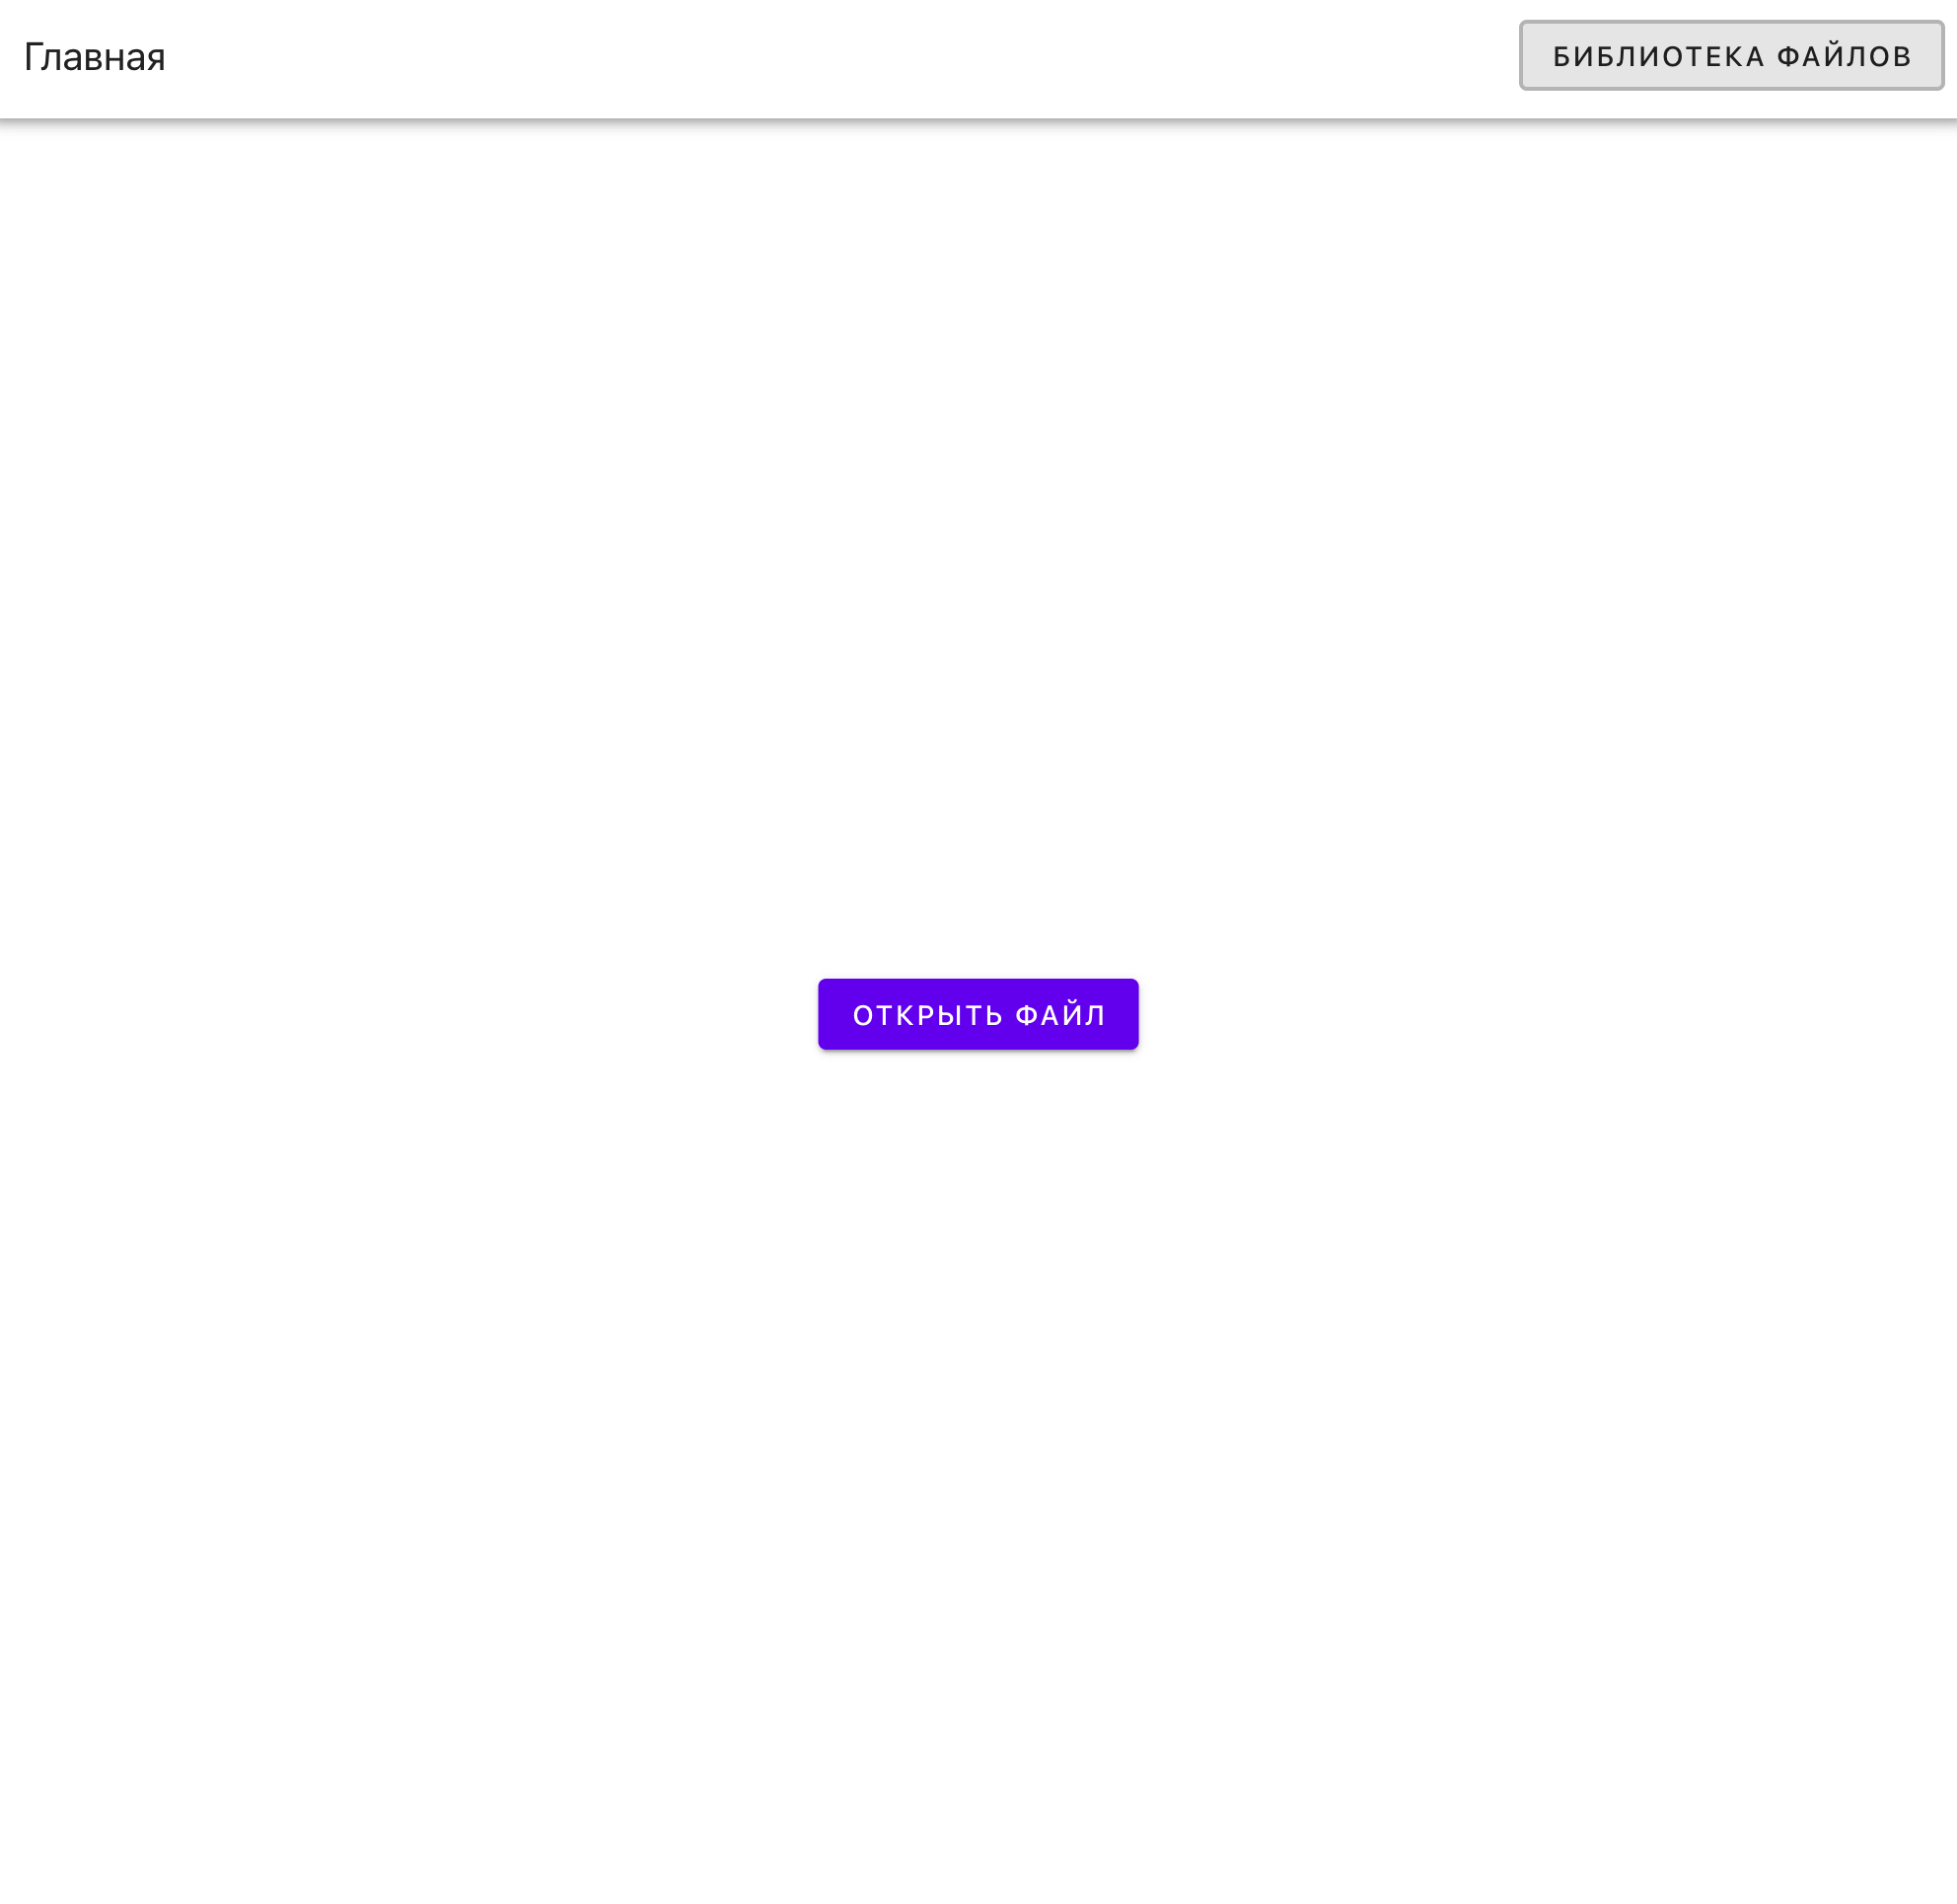
\includegraphics[width=0.65\textwidth]{startup}}}
  \caption{Интерфейс программы при запуске}
  \label{ris:startup}
\end{figure}


\begin{figure}[H]
  \center{\frame{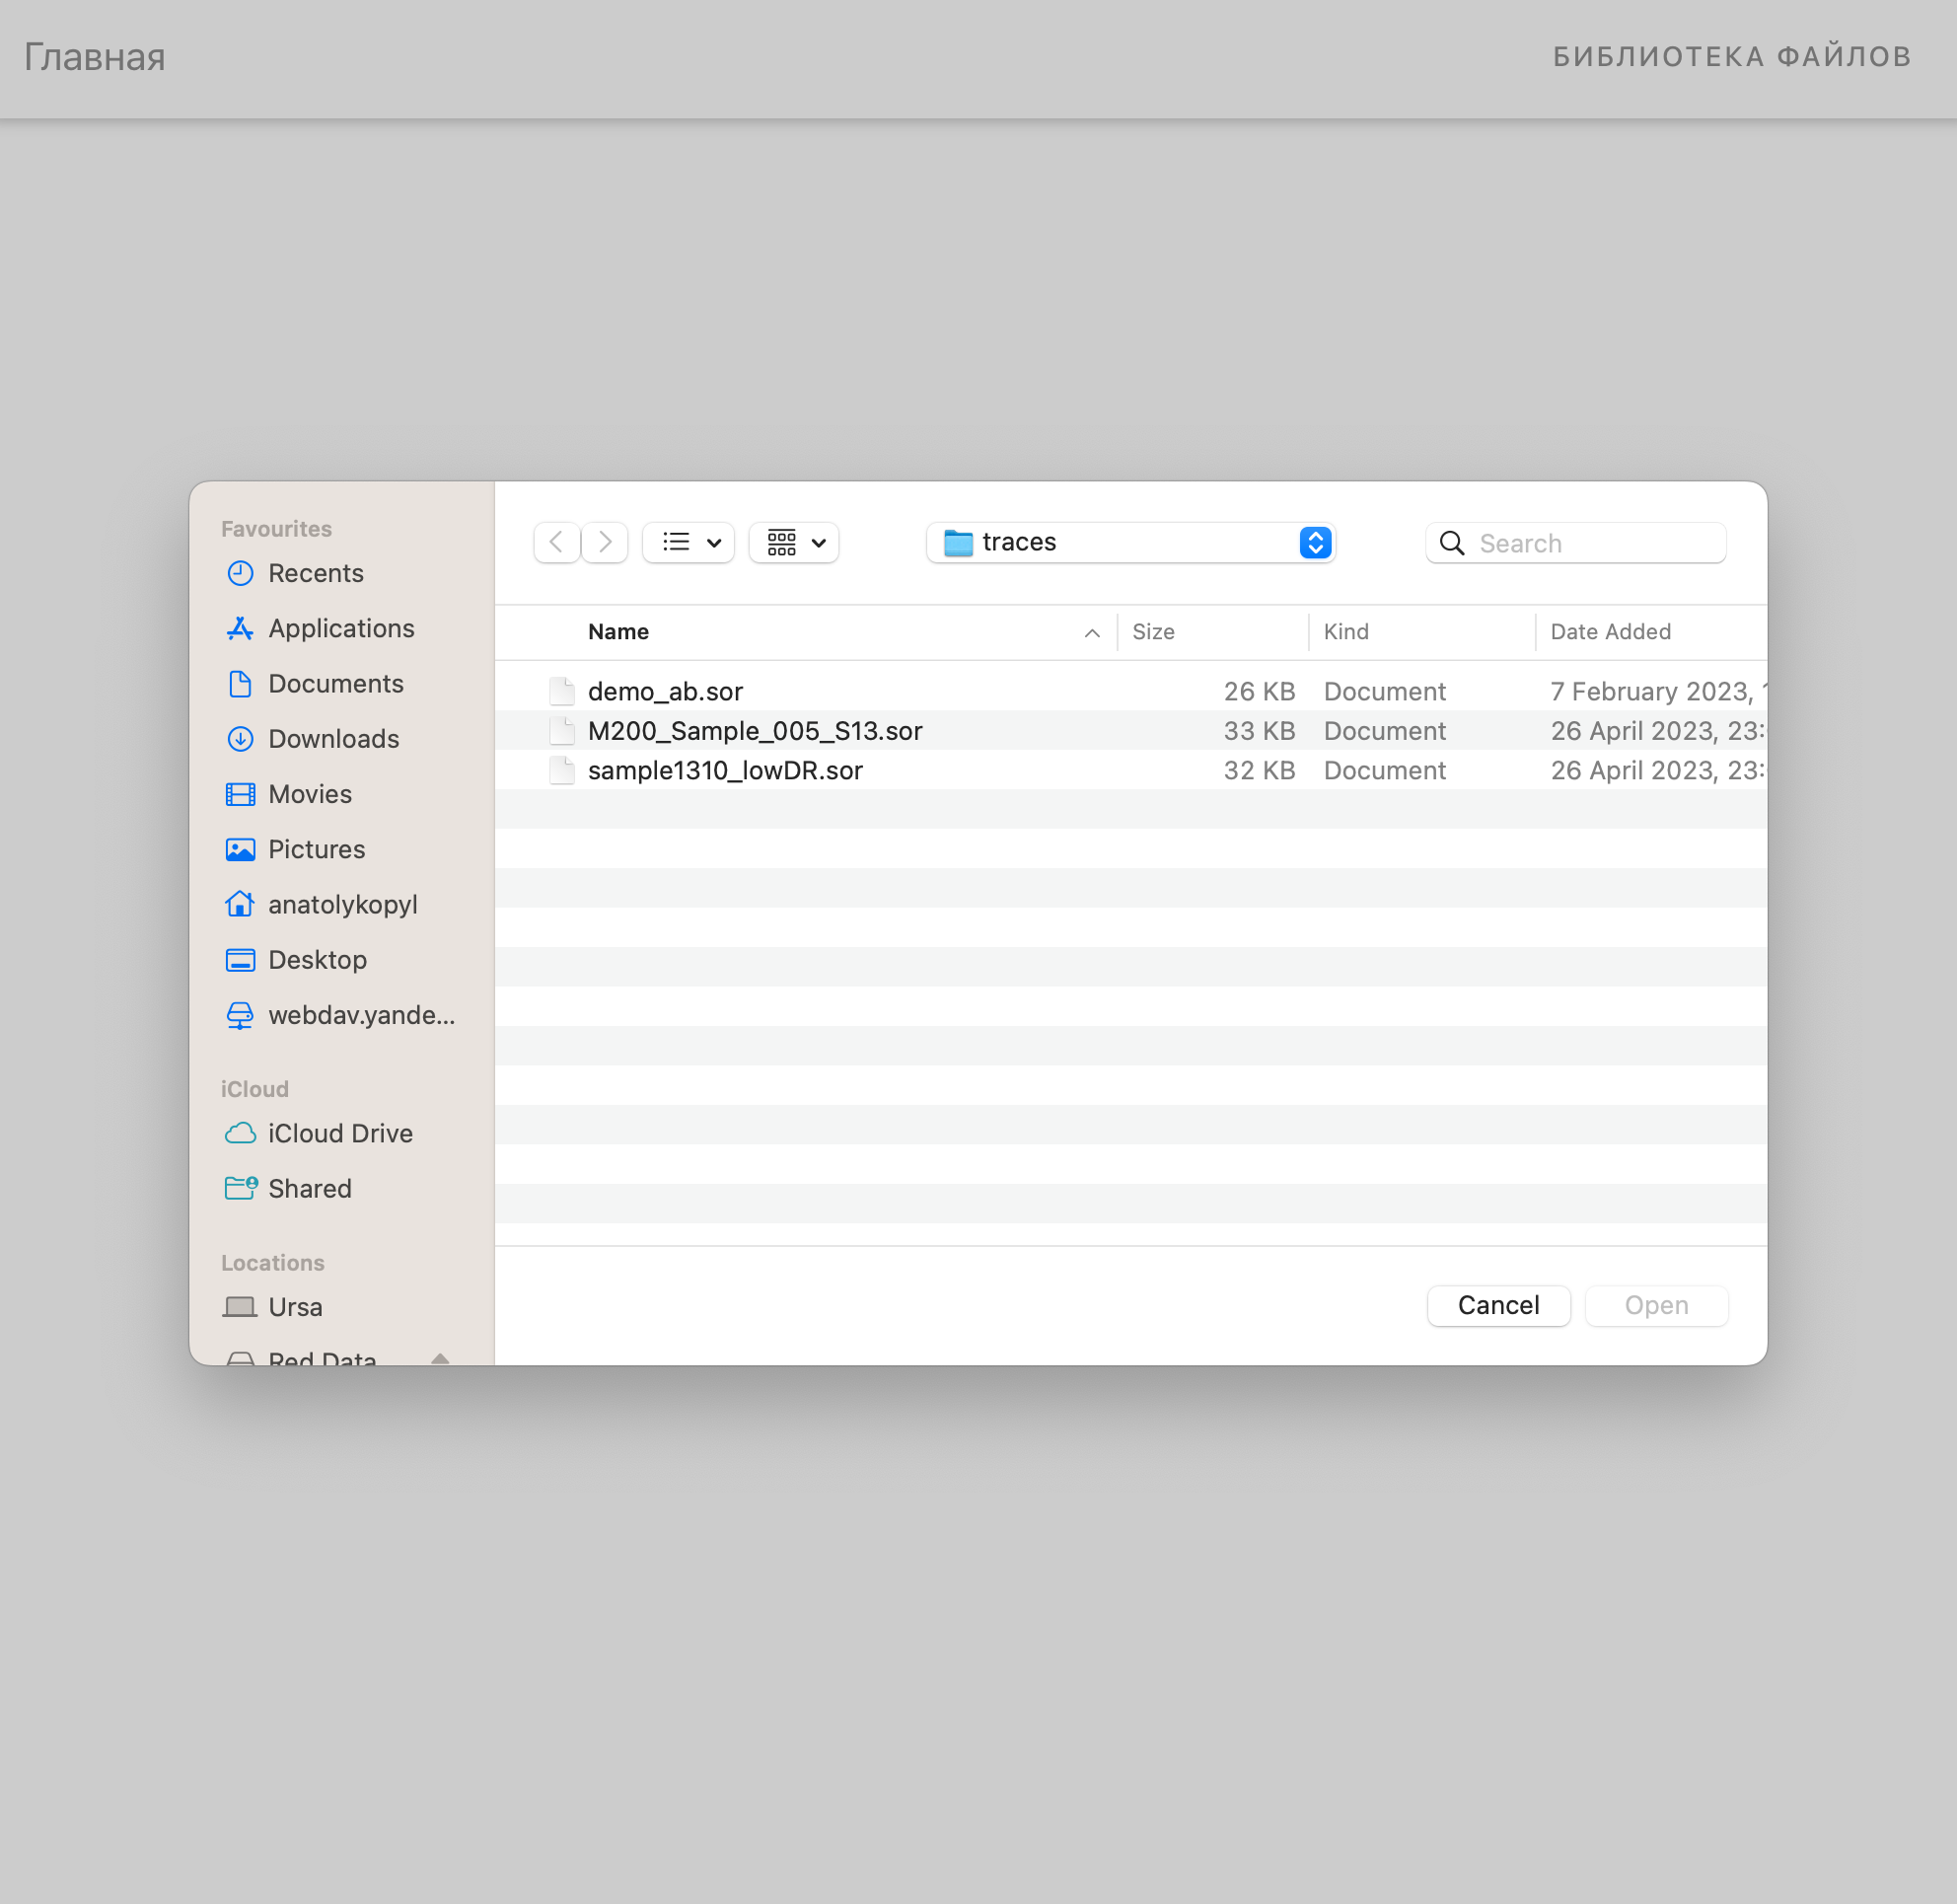
\includegraphics[width=0.65\textwidth]{file_manager}}}
  \caption{Файловый менеджер}
  \label{ris:file_manager}
\end{figure}

\begin{figure}[H]
  \center{\frame{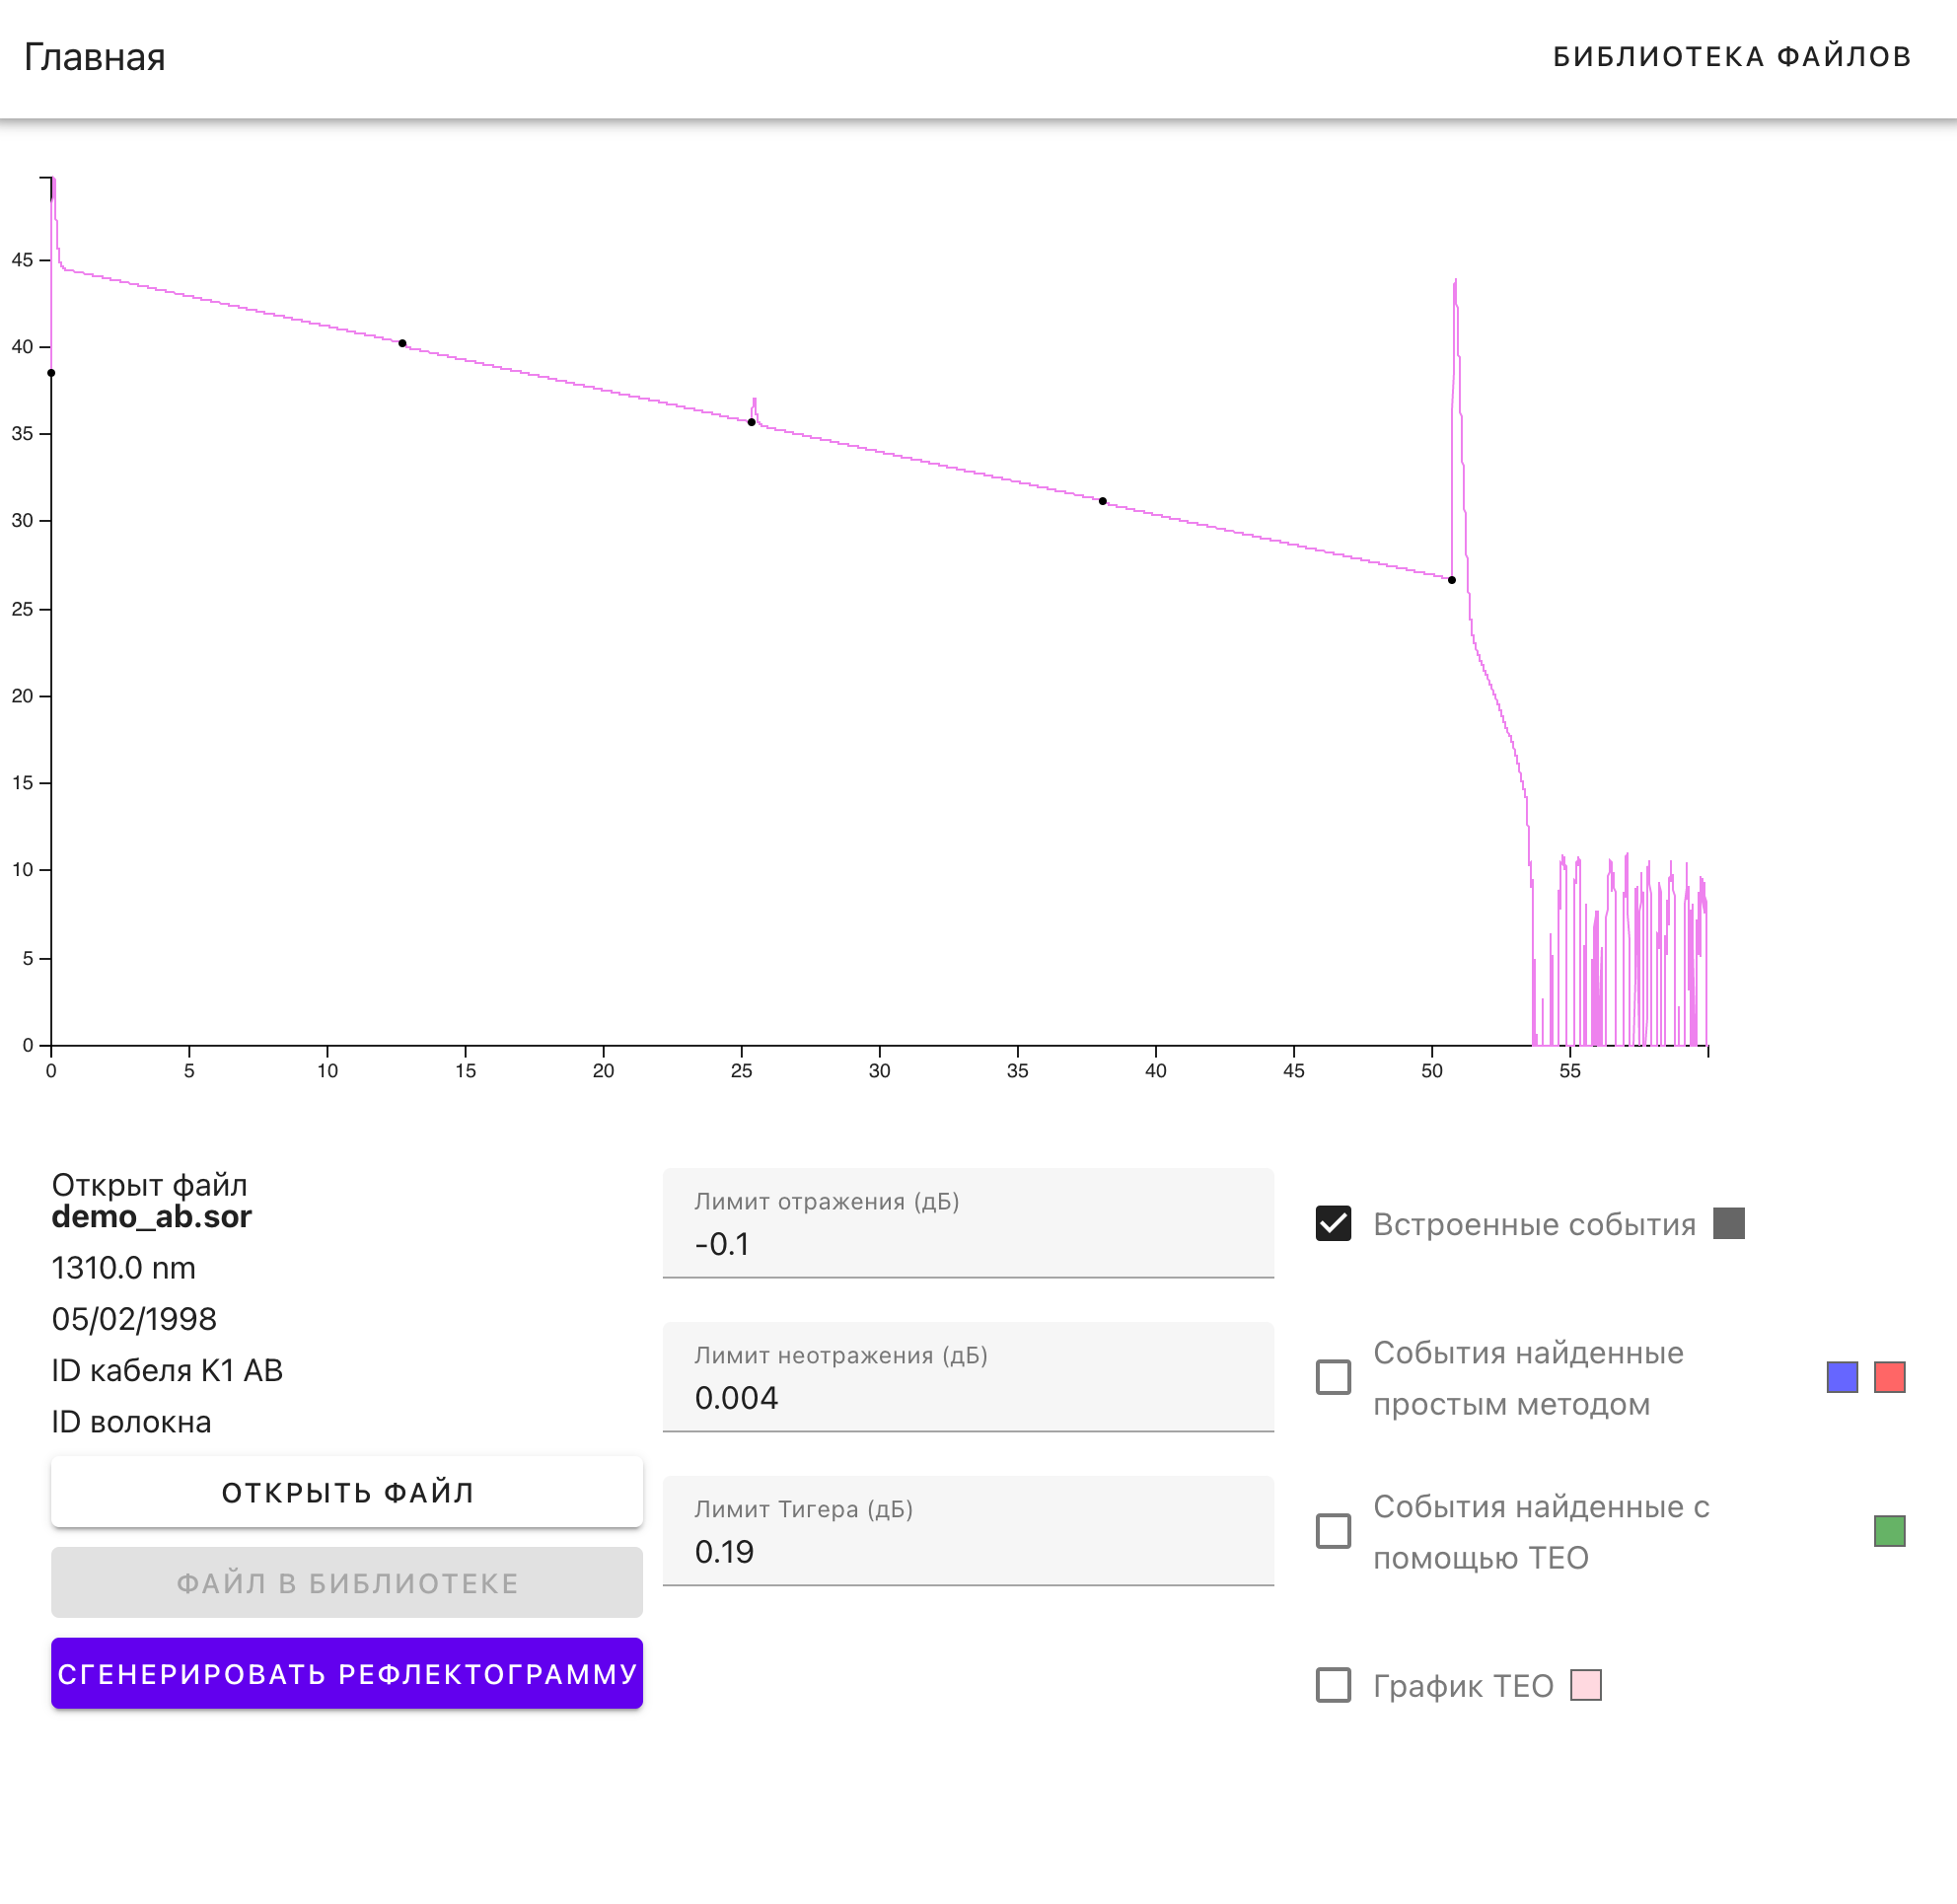
\includegraphics[width=0.65\textwidth]{opened_file}}}
  \caption{Файл открыт}
  \label{ris:opened_file}
\end{figure}

\subsection{Функция <<Поиск событий>>}

\begin{figure}[H]
  \center{\frame{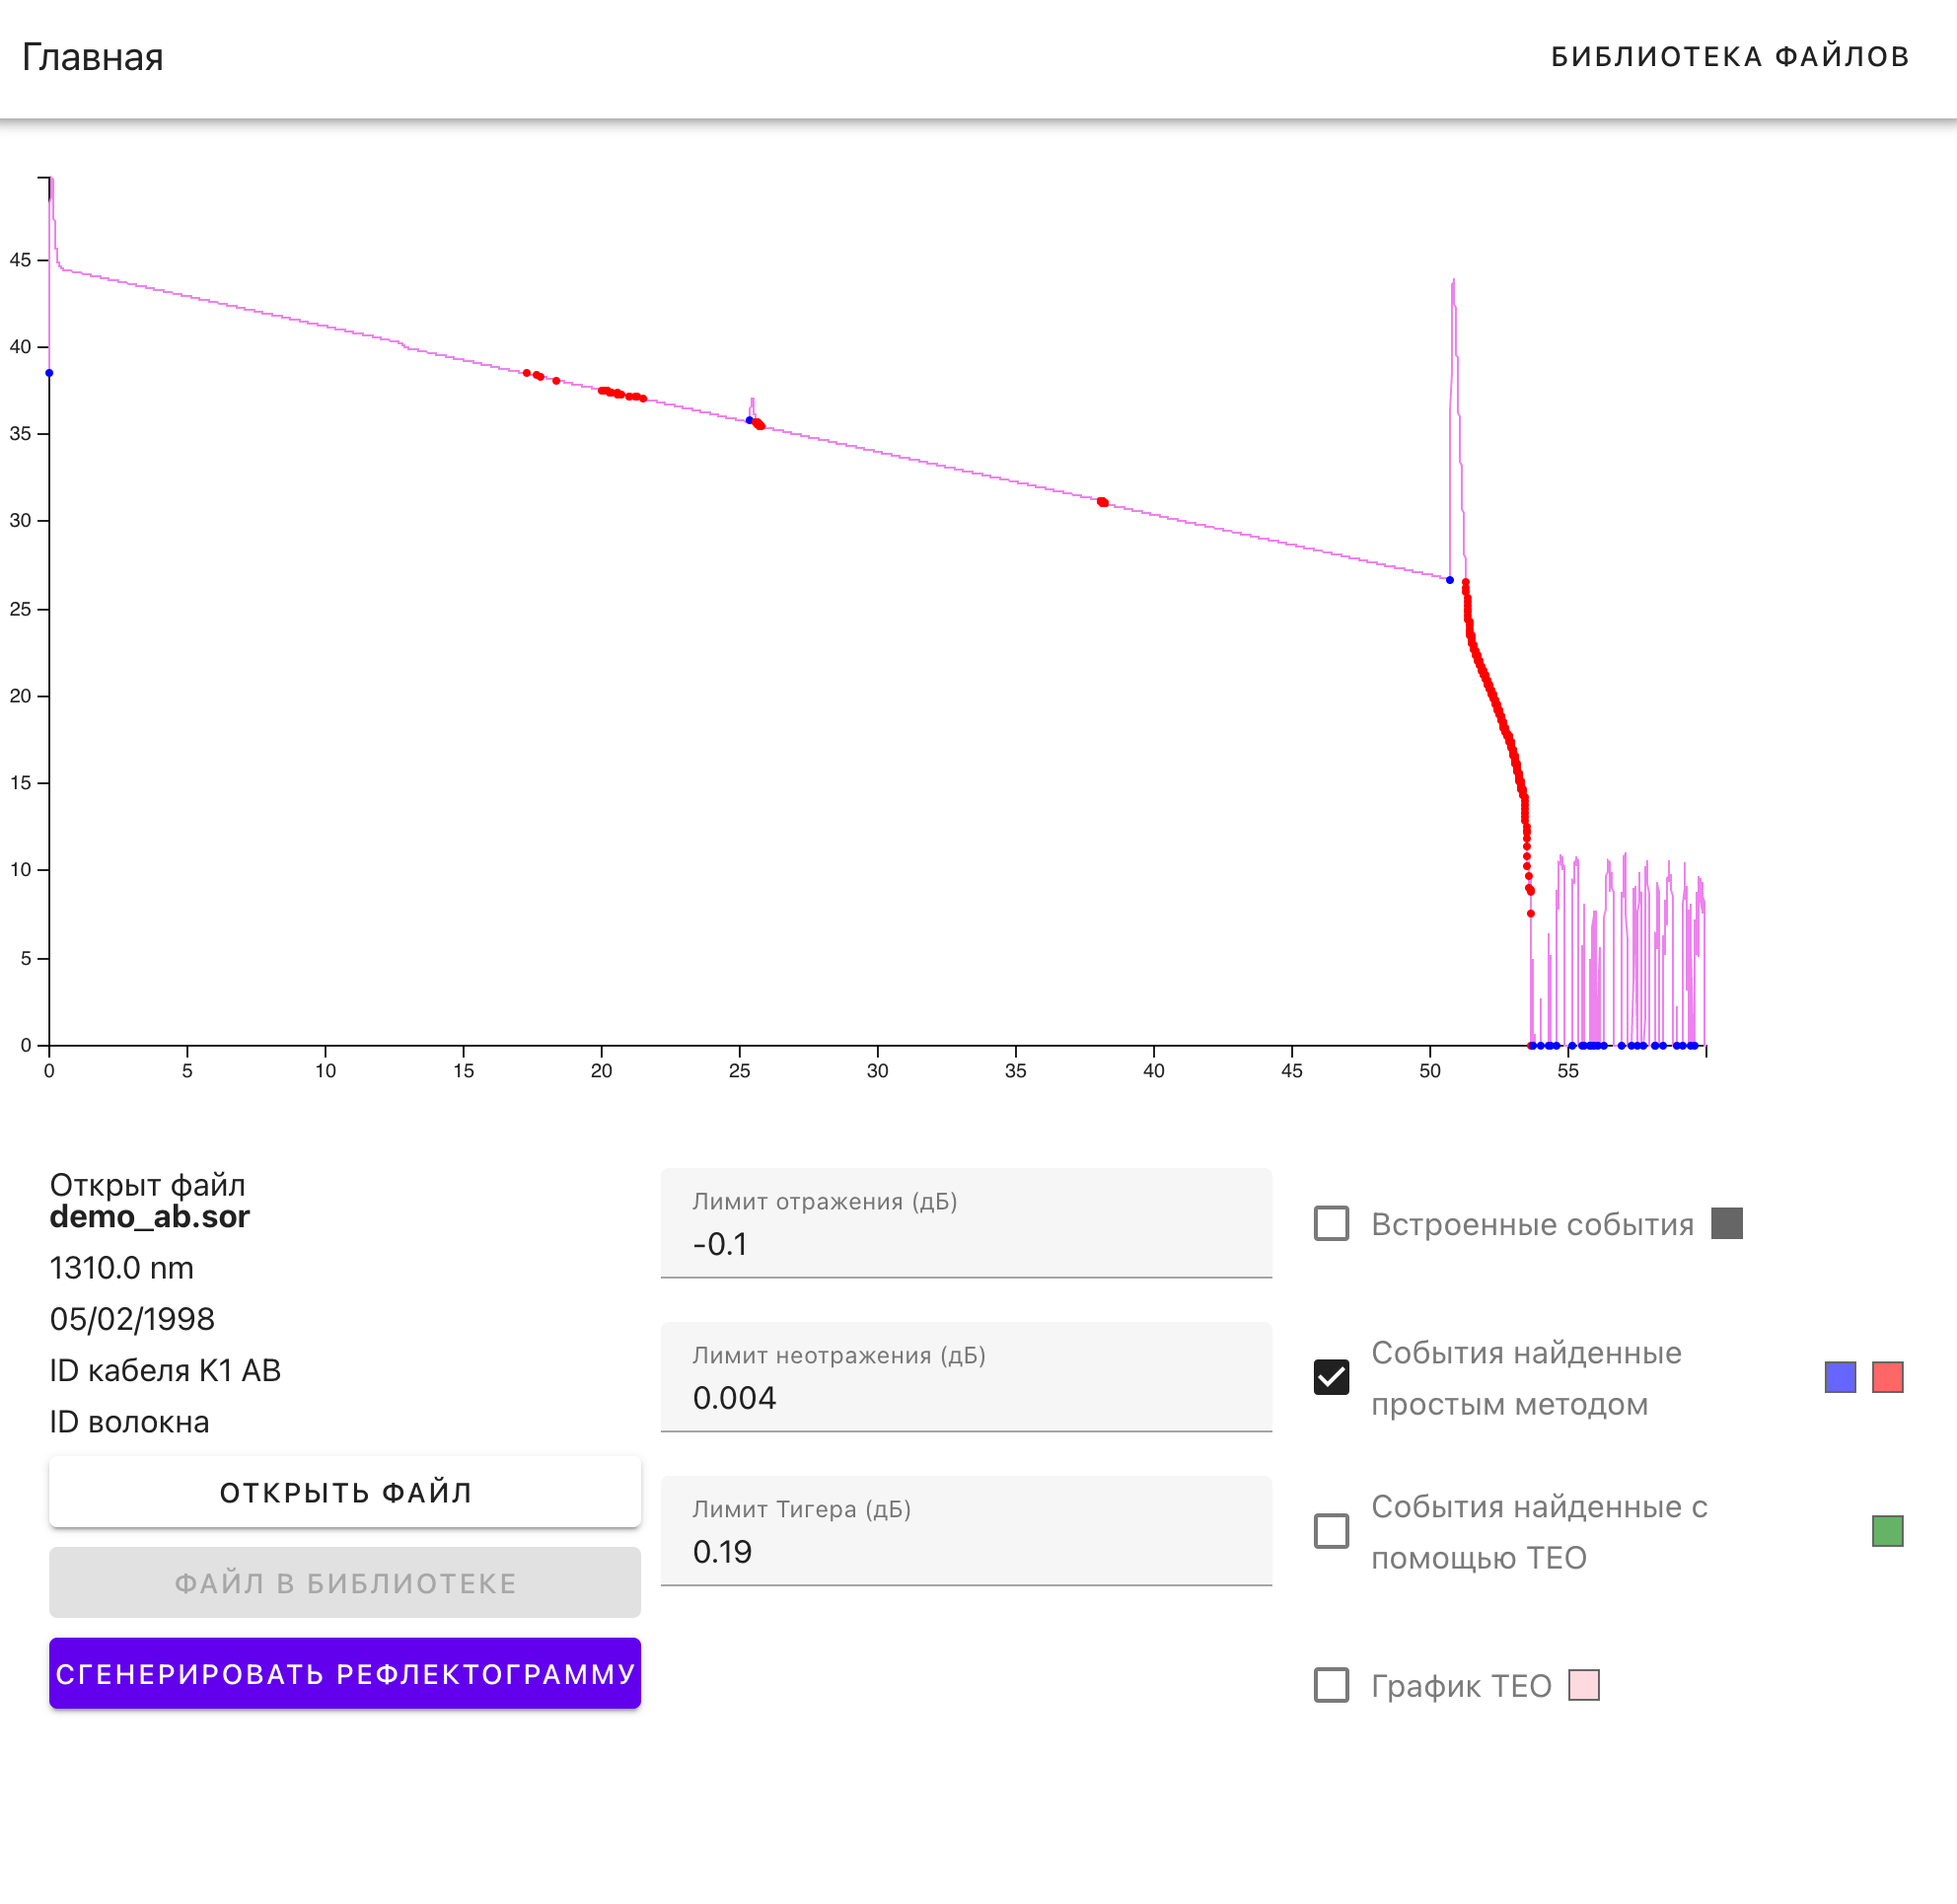
\includegraphics[width=0.65\textwidth]{naive_events}}}
  \caption{События найденные простым алгоритмом}
  \label{ris:naive_events}
\end{figure}

\begin{figure}[H]
  \center{\frame{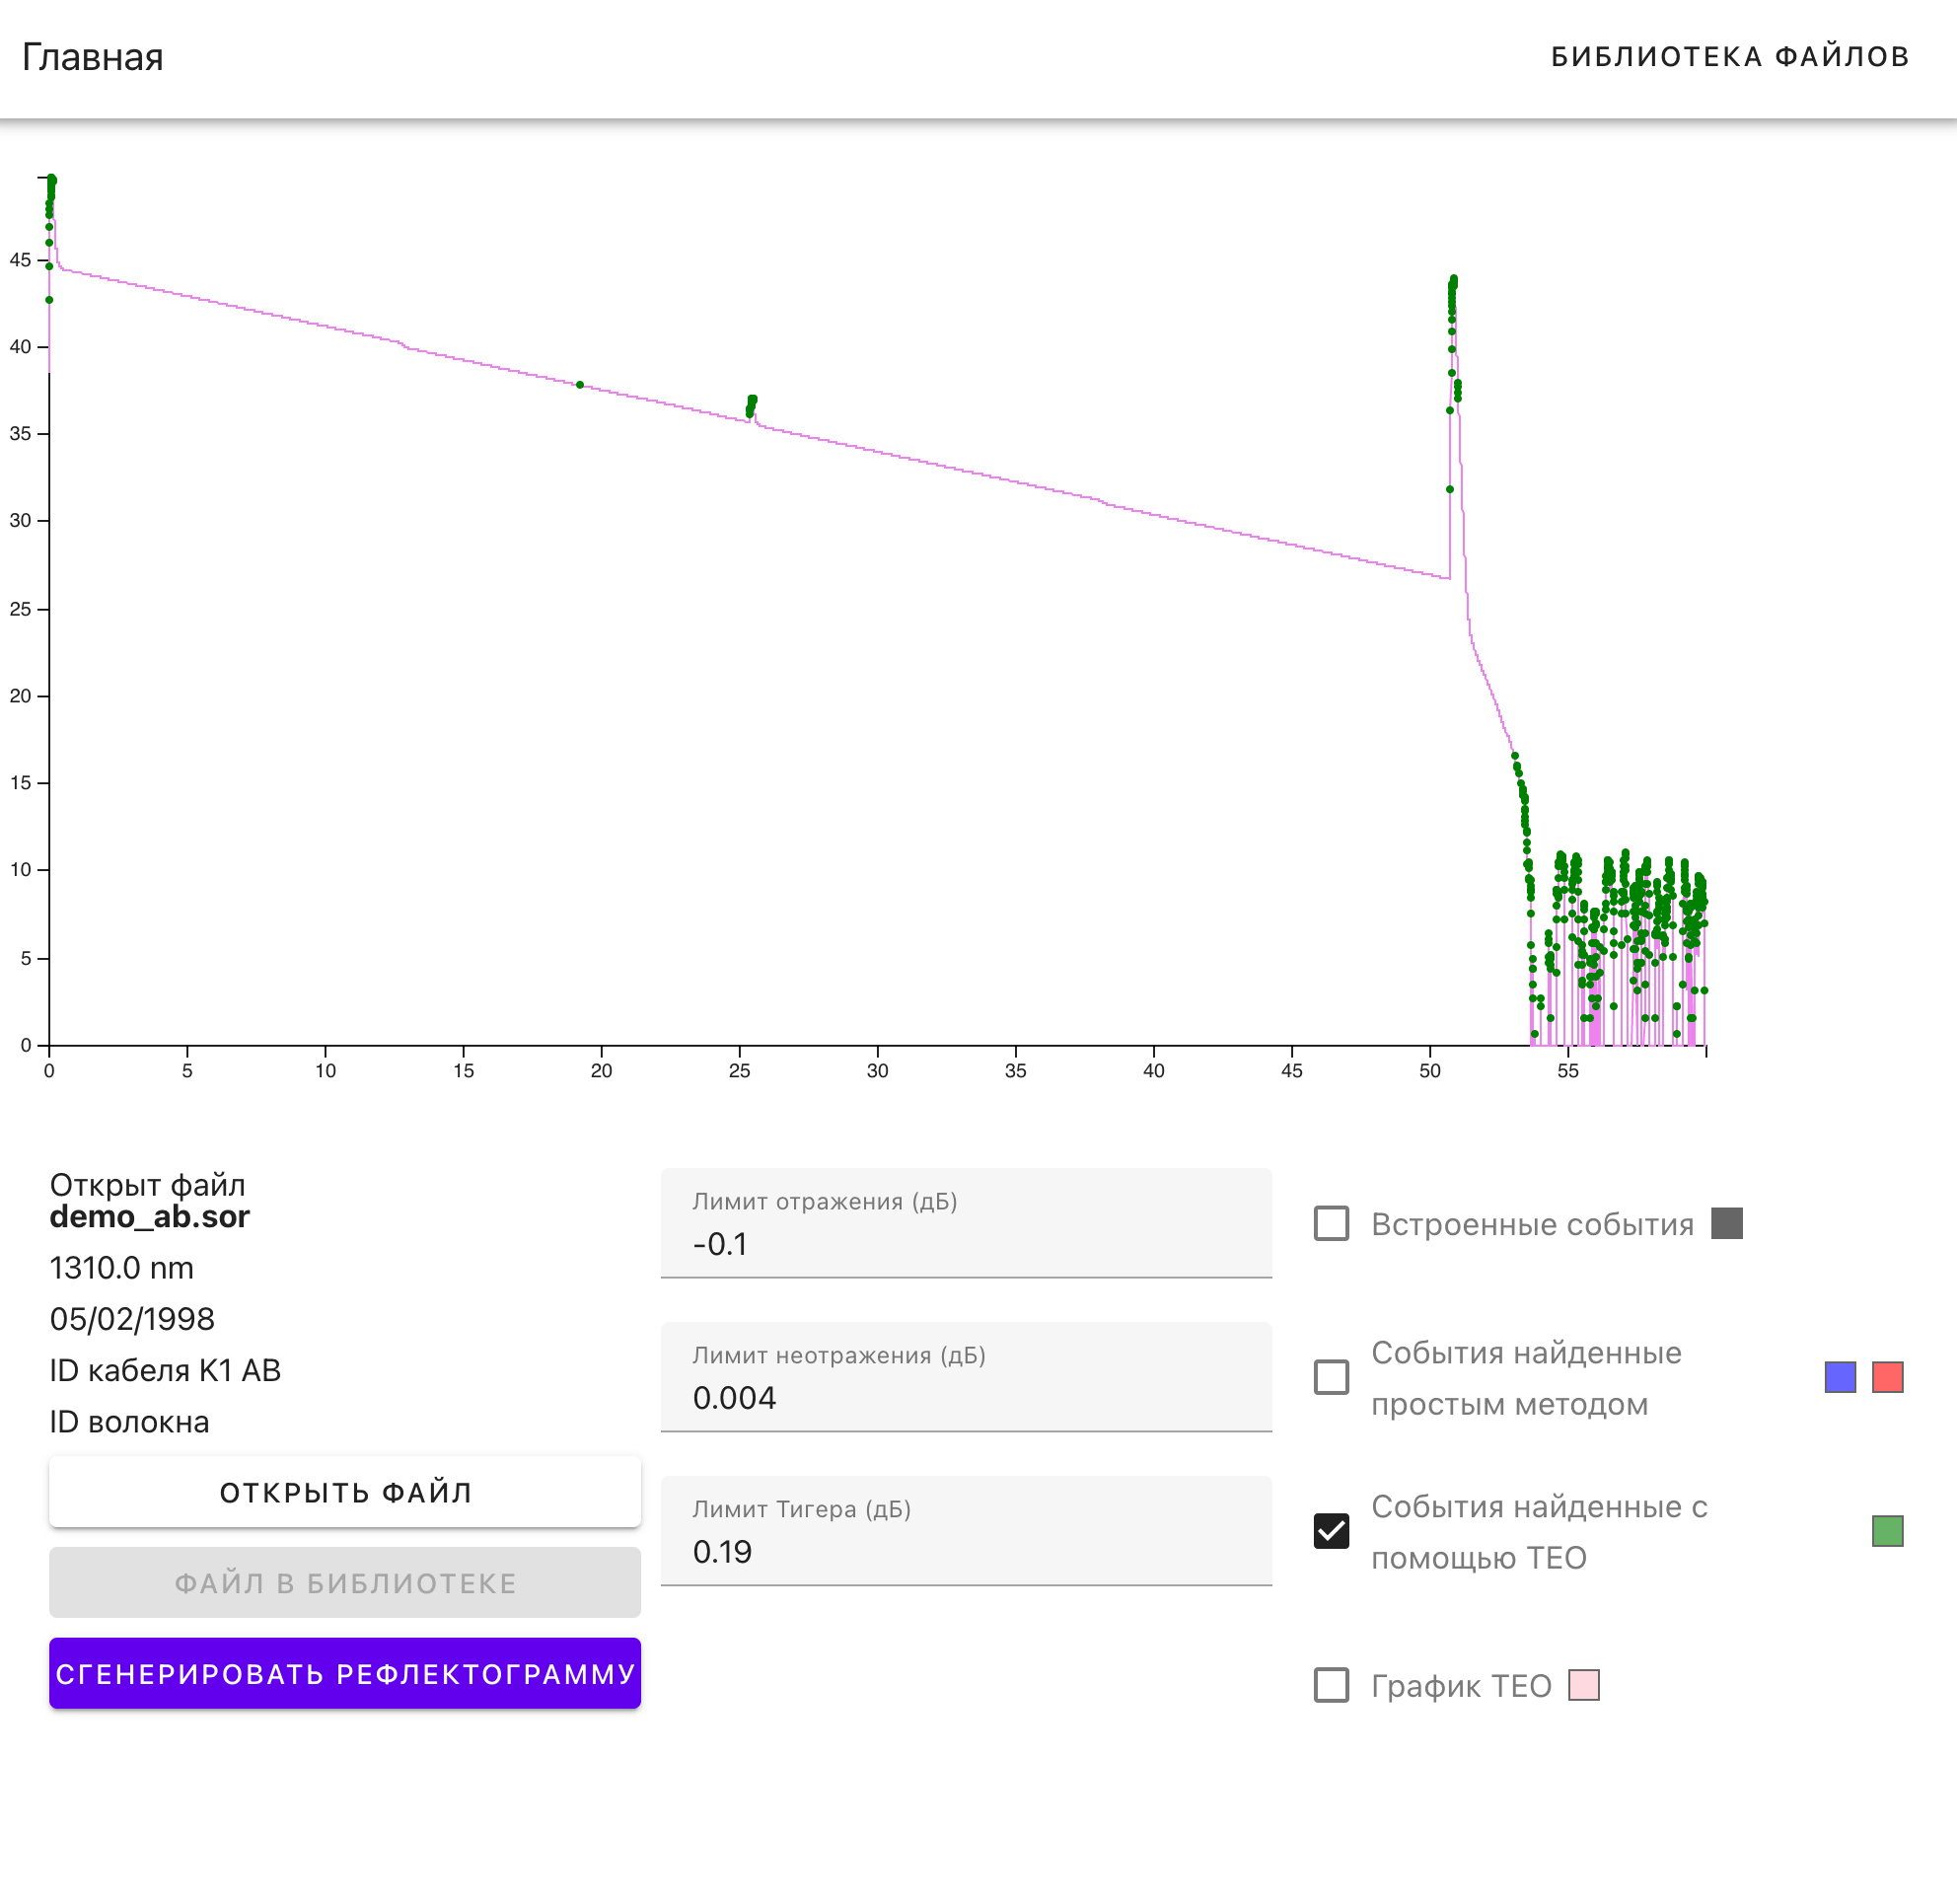
\includegraphics[width=0.65\textwidth]{teo_events}}}
  \caption{События найденные алгоритмом на основе \acrshort{teo}}
  \label{ris:teo_events}
\end{figure}

\begin{figure}[H]
  \center{\frame{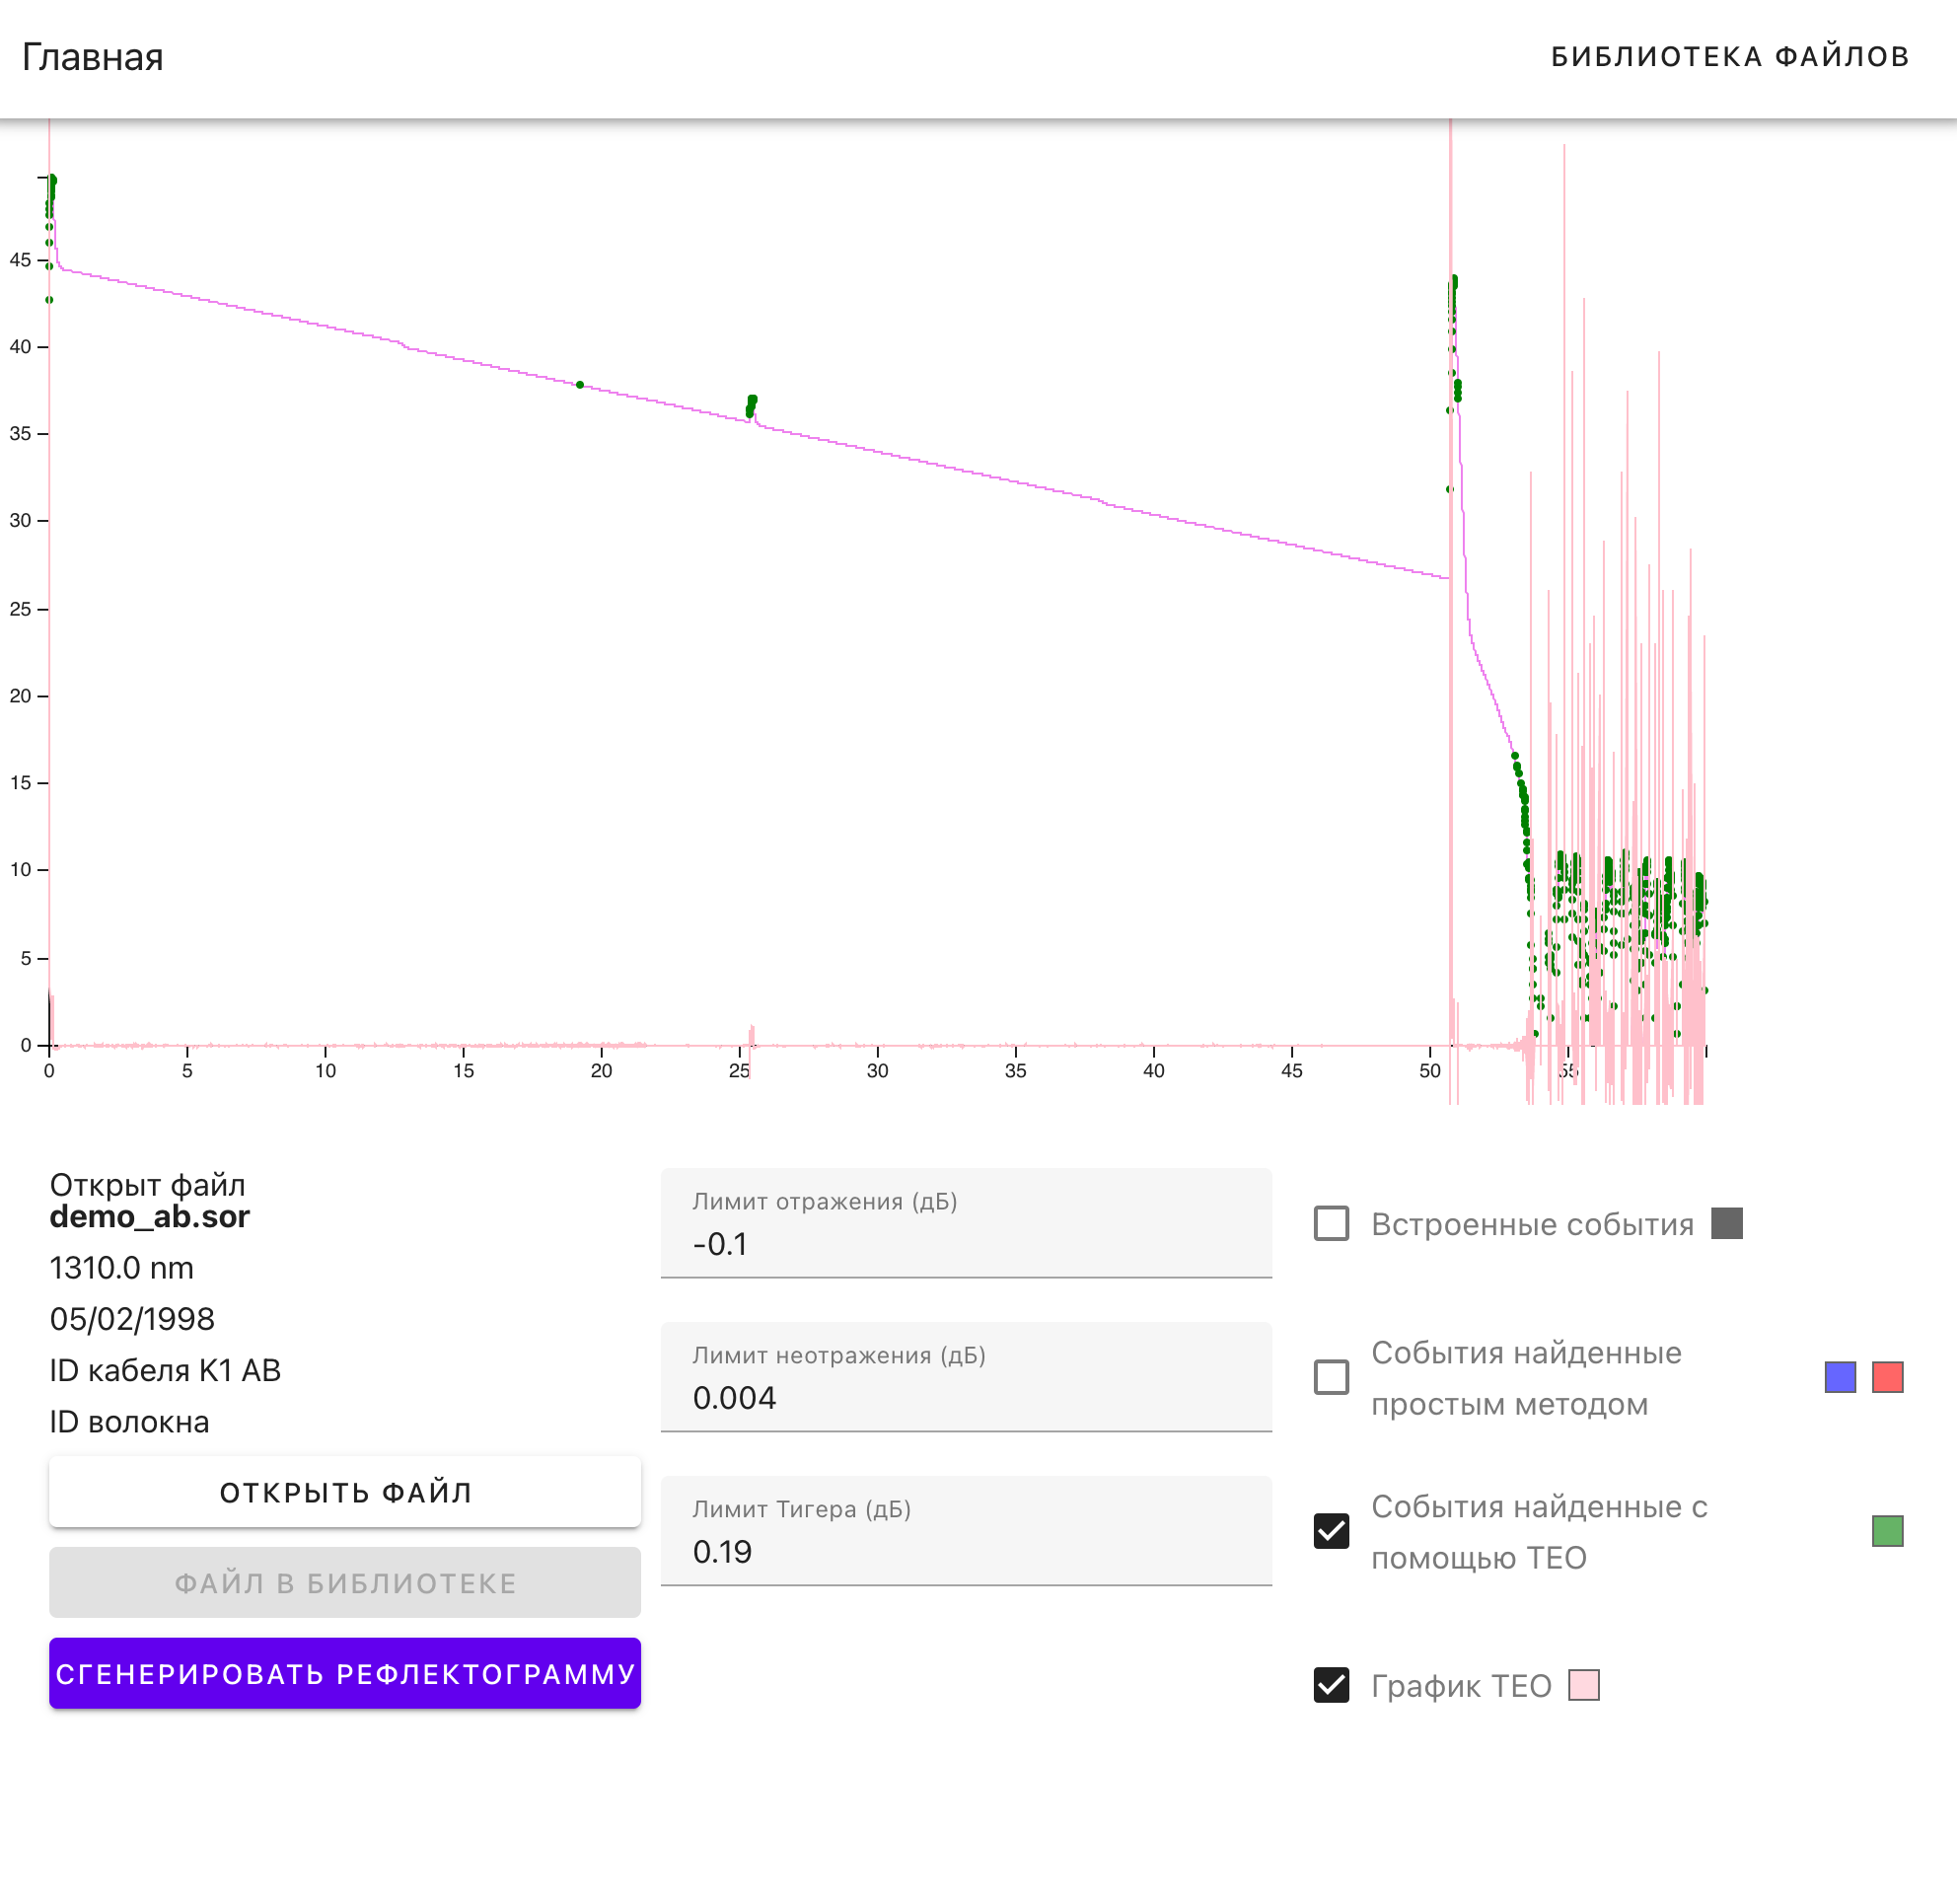
\includegraphics[width=0.65\textwidth]{teo_events_and_values}}}
  \caption{События найденные алгоритмом на основе \acrshort{teo} и график значений \acrshort{teo}}
  \label{ris:teo_events_and_values}
\end{figure}

\begin{figure}[H]
  \center{\frame{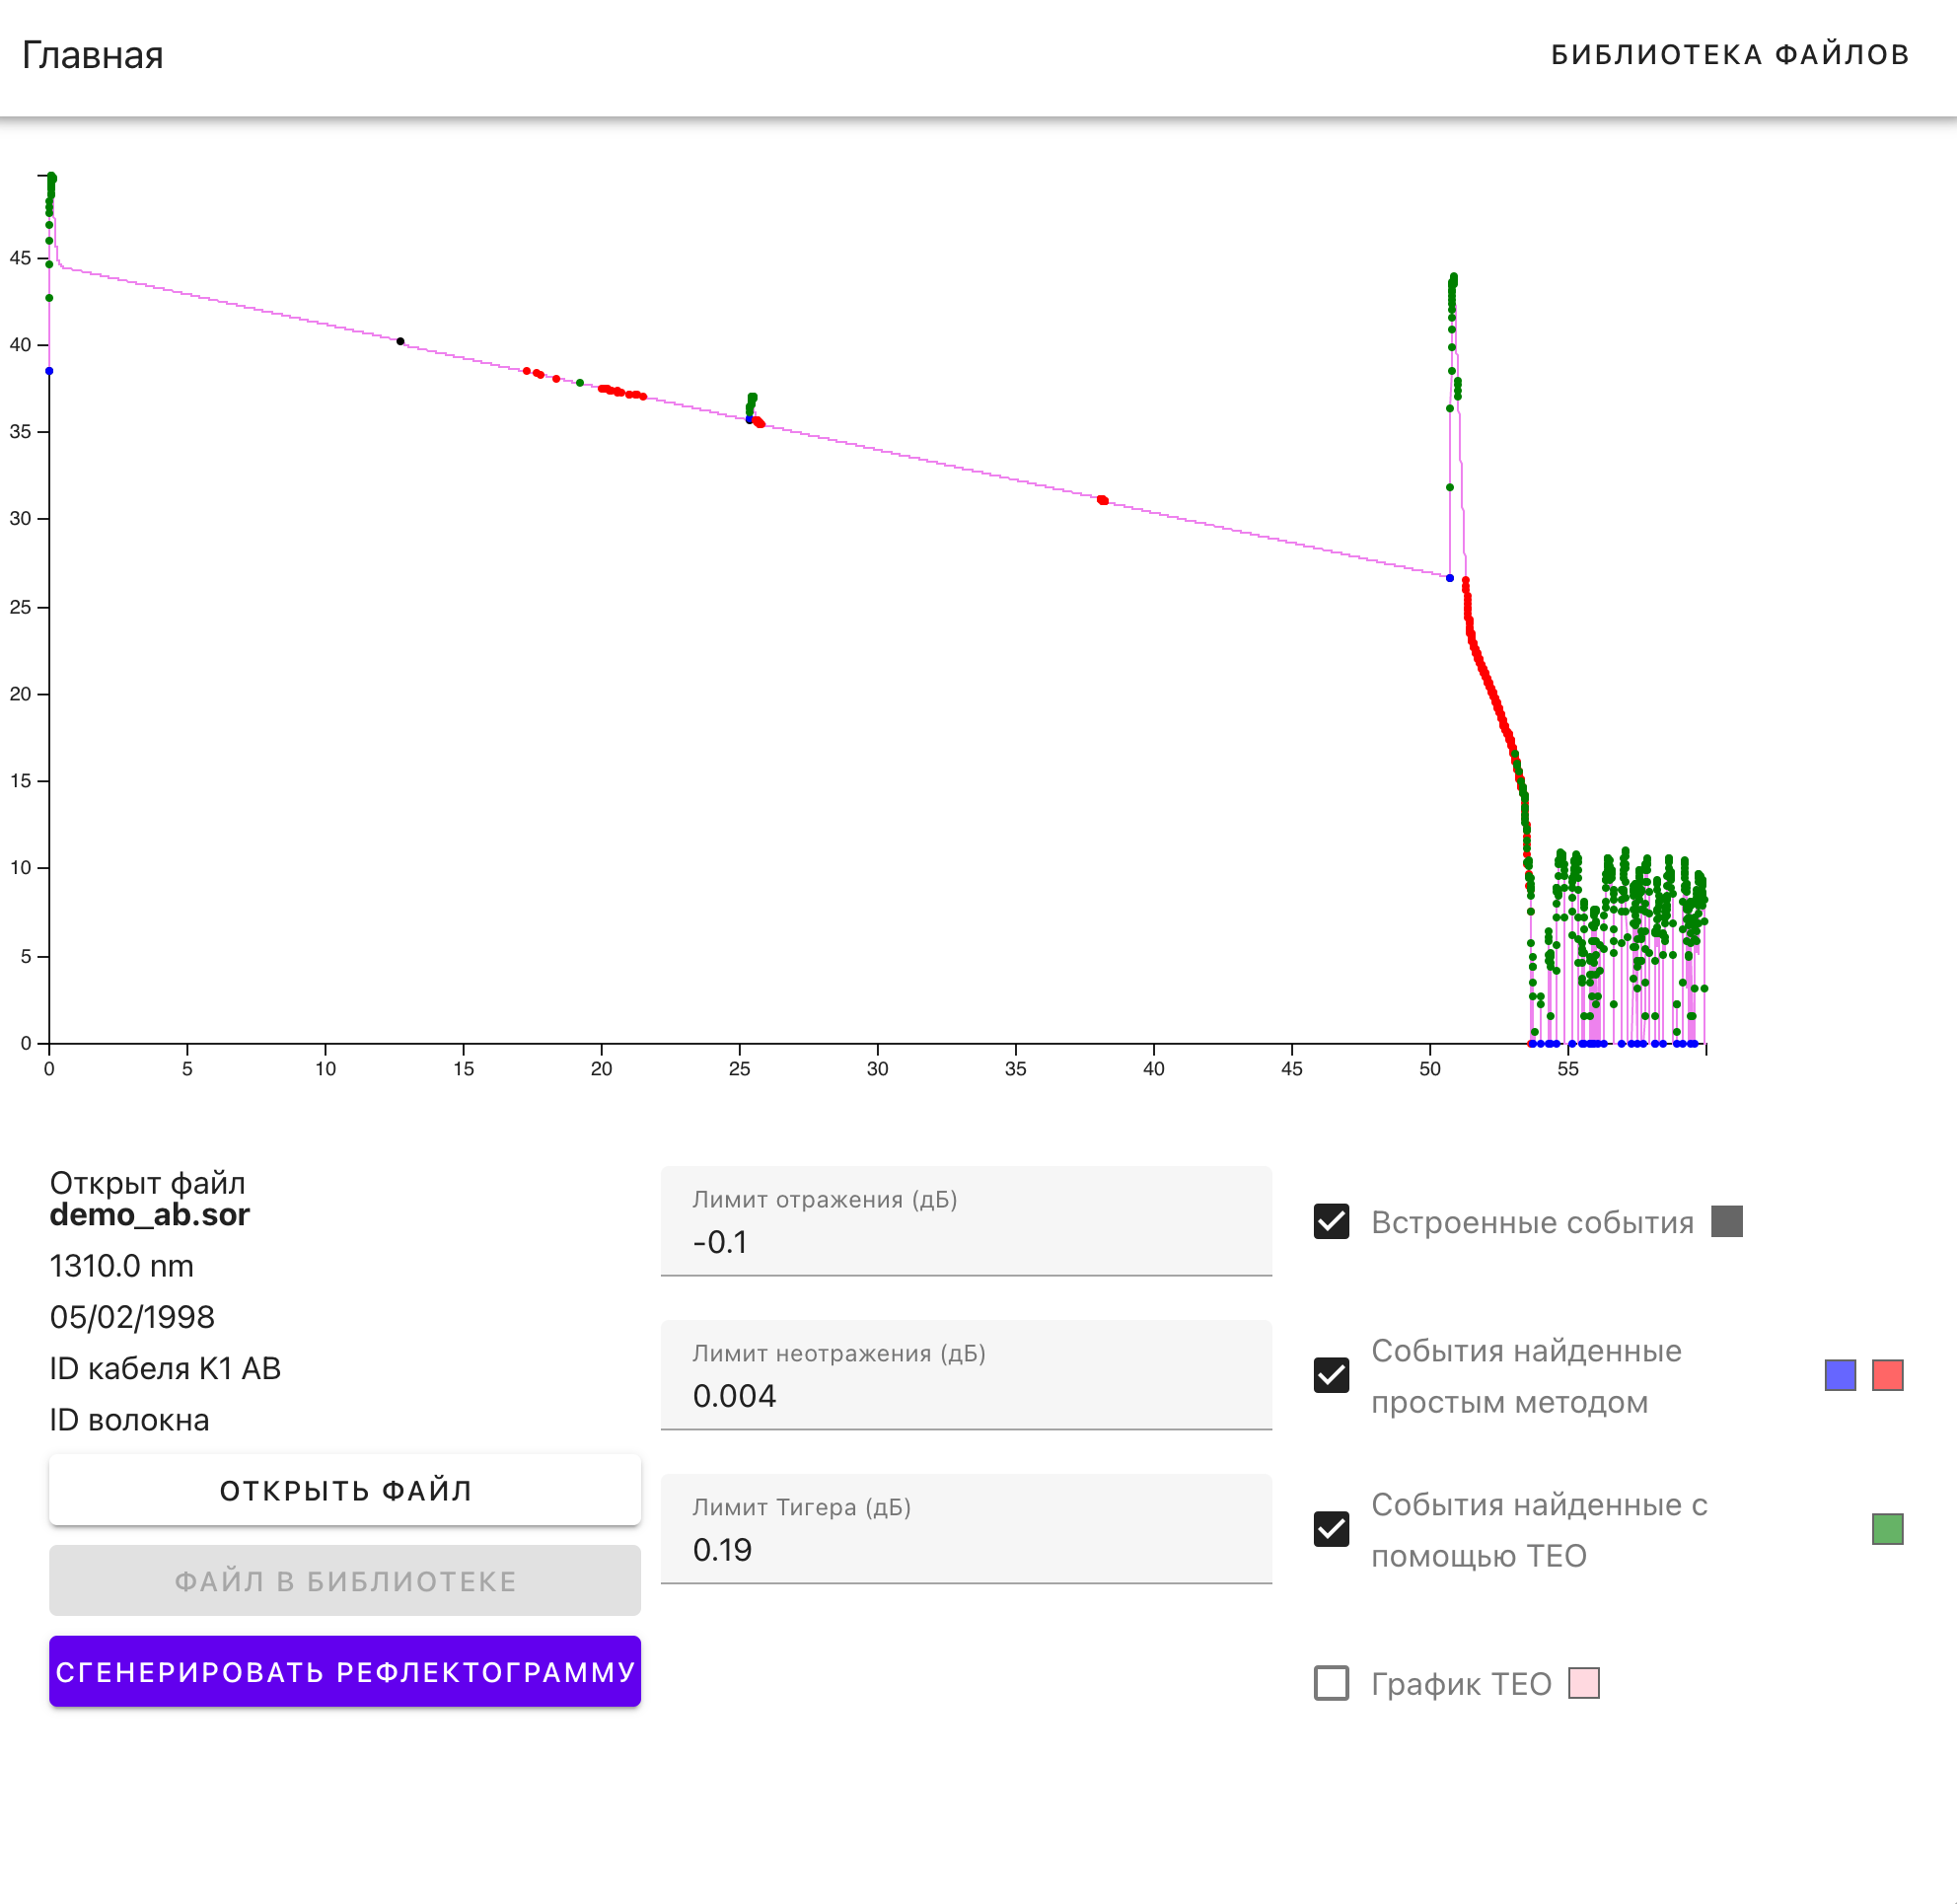
\includegraphics[width=0.65\textwidth]{all_events}}}
  \caption{Все найденные события}
  \label{ris:all_events}
\end{figure}

\subsection{Функция <<Встроенная библиотека>>}

\begin{figure}[H]
  \center{\frame{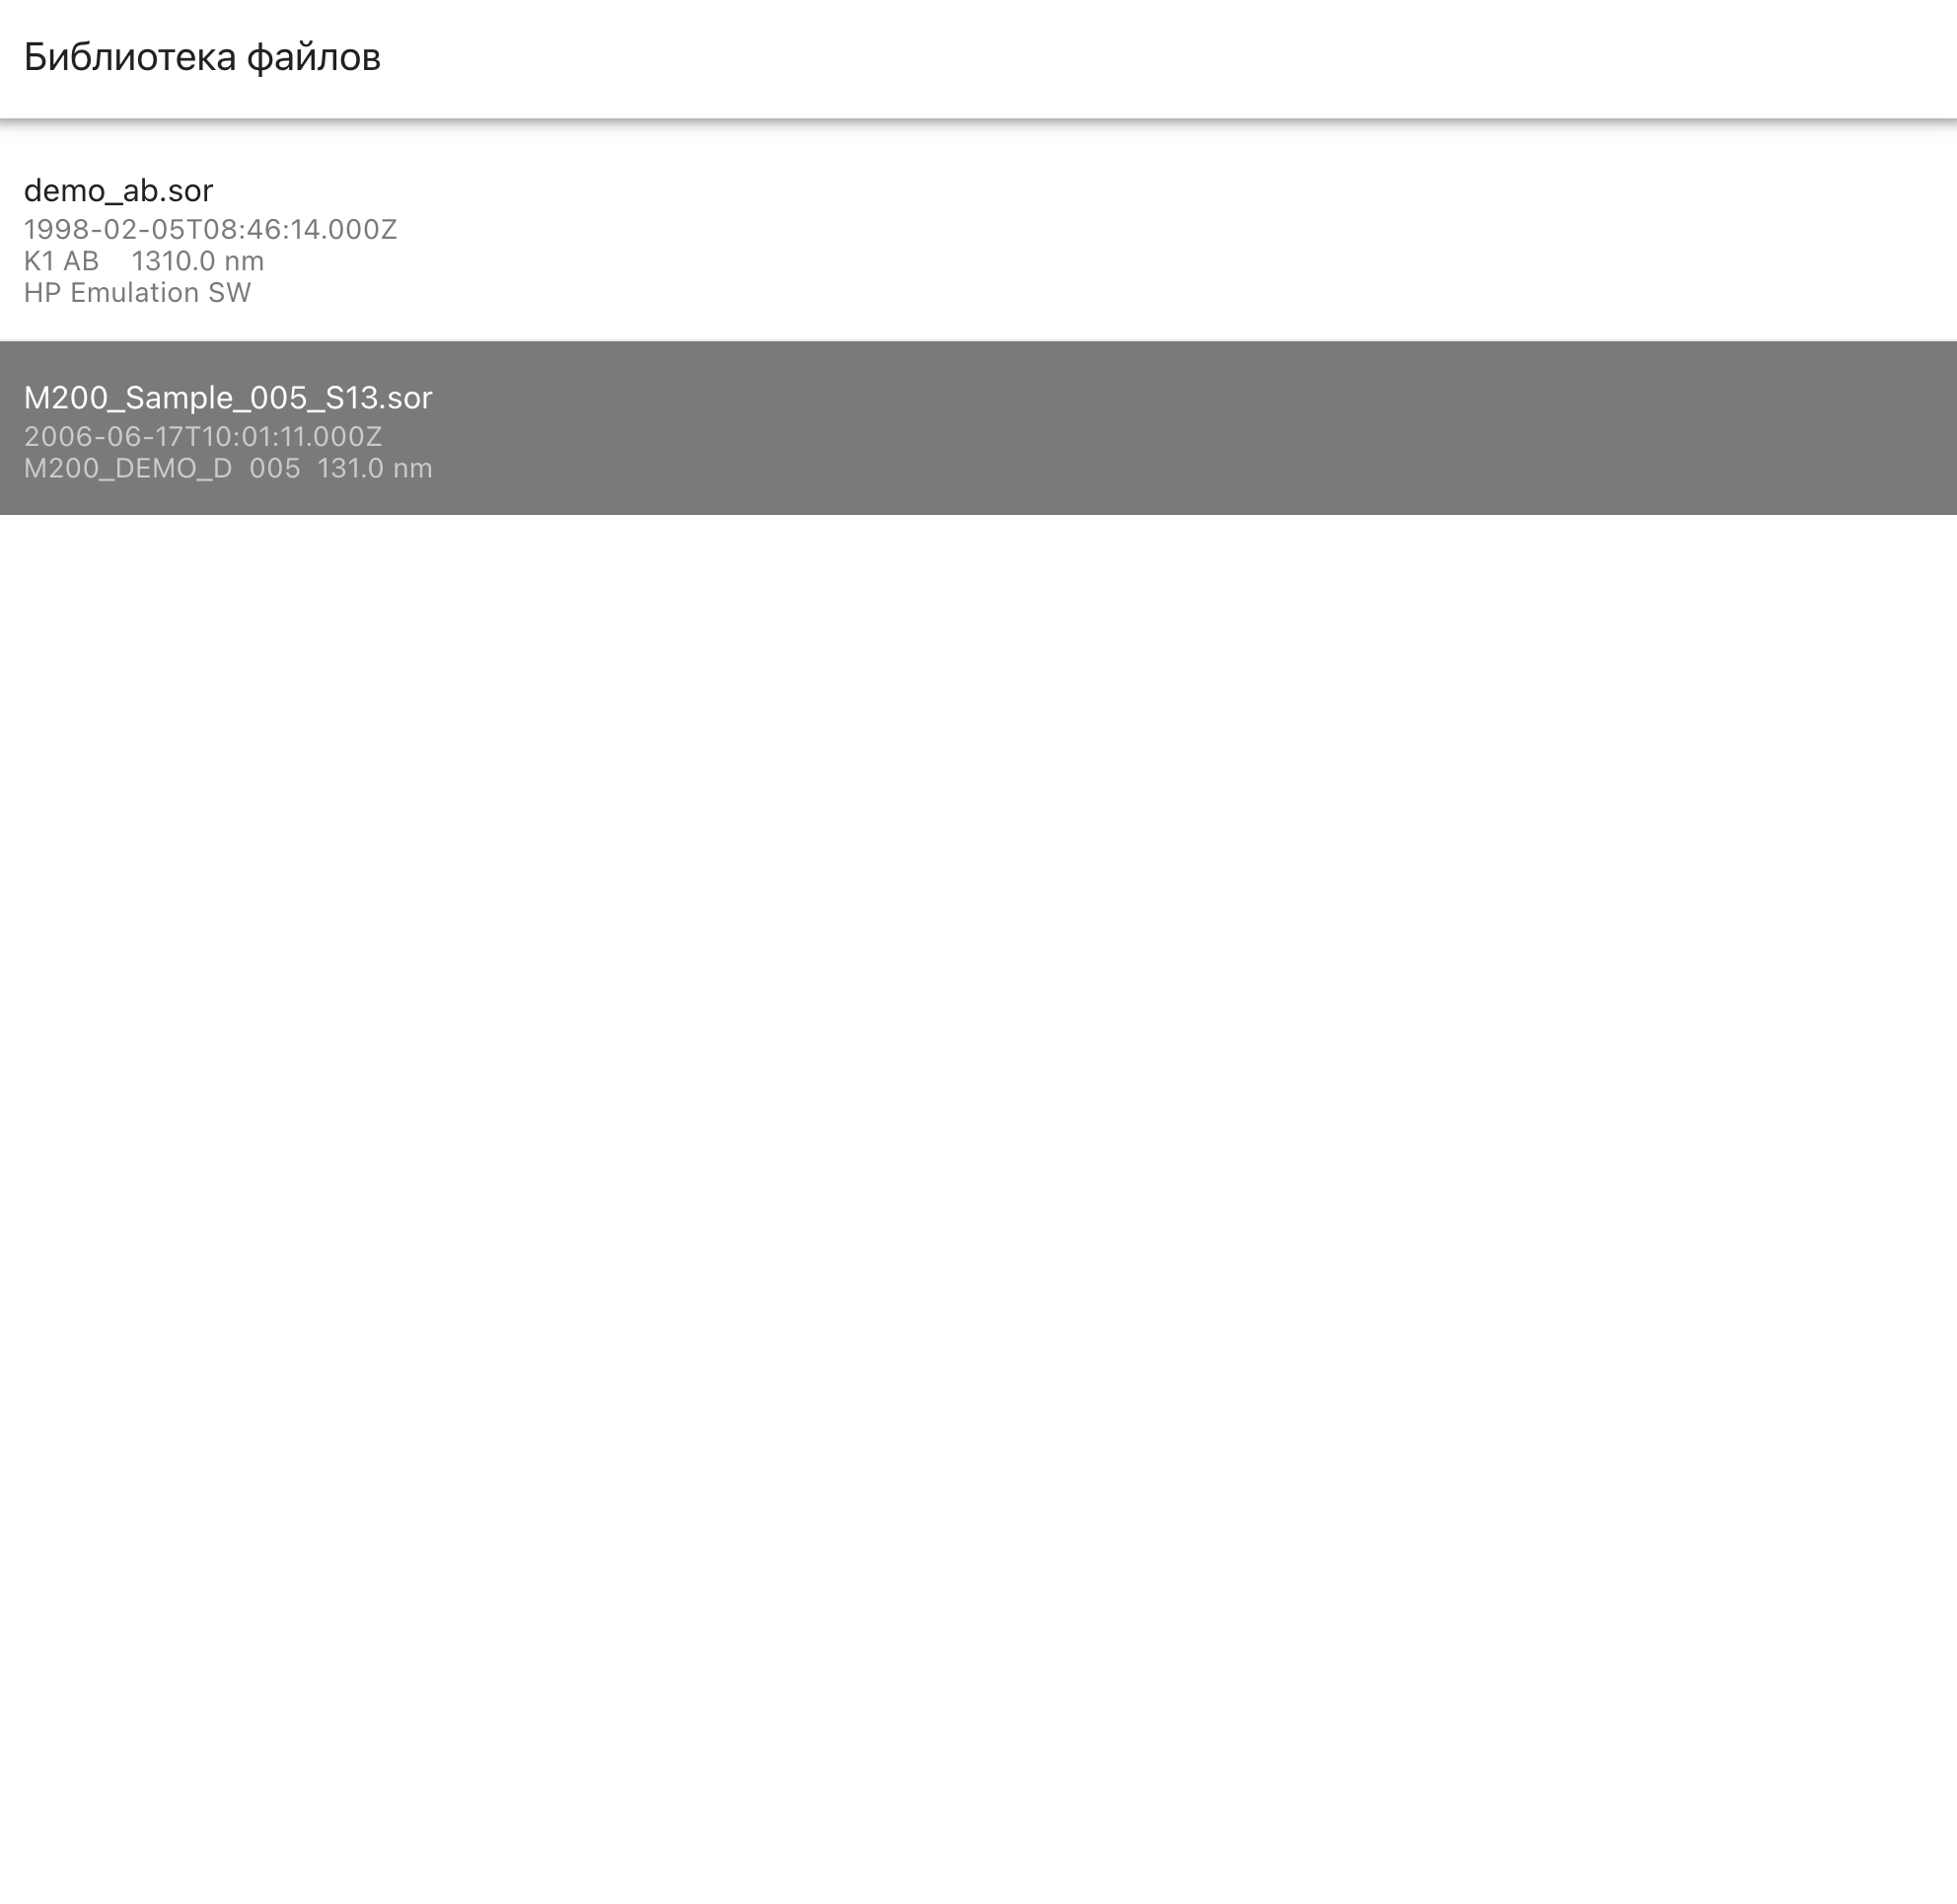
\includegraphics[width=0.65\textwidth]{library}}}
  \caption{Библиотека рефлектограмм}
  \label{ris:library}
\end{figure}

\subsection{Функция <<Редактирование рефлектограммы>>}

\begin{figure}[H]
  \center{\frame{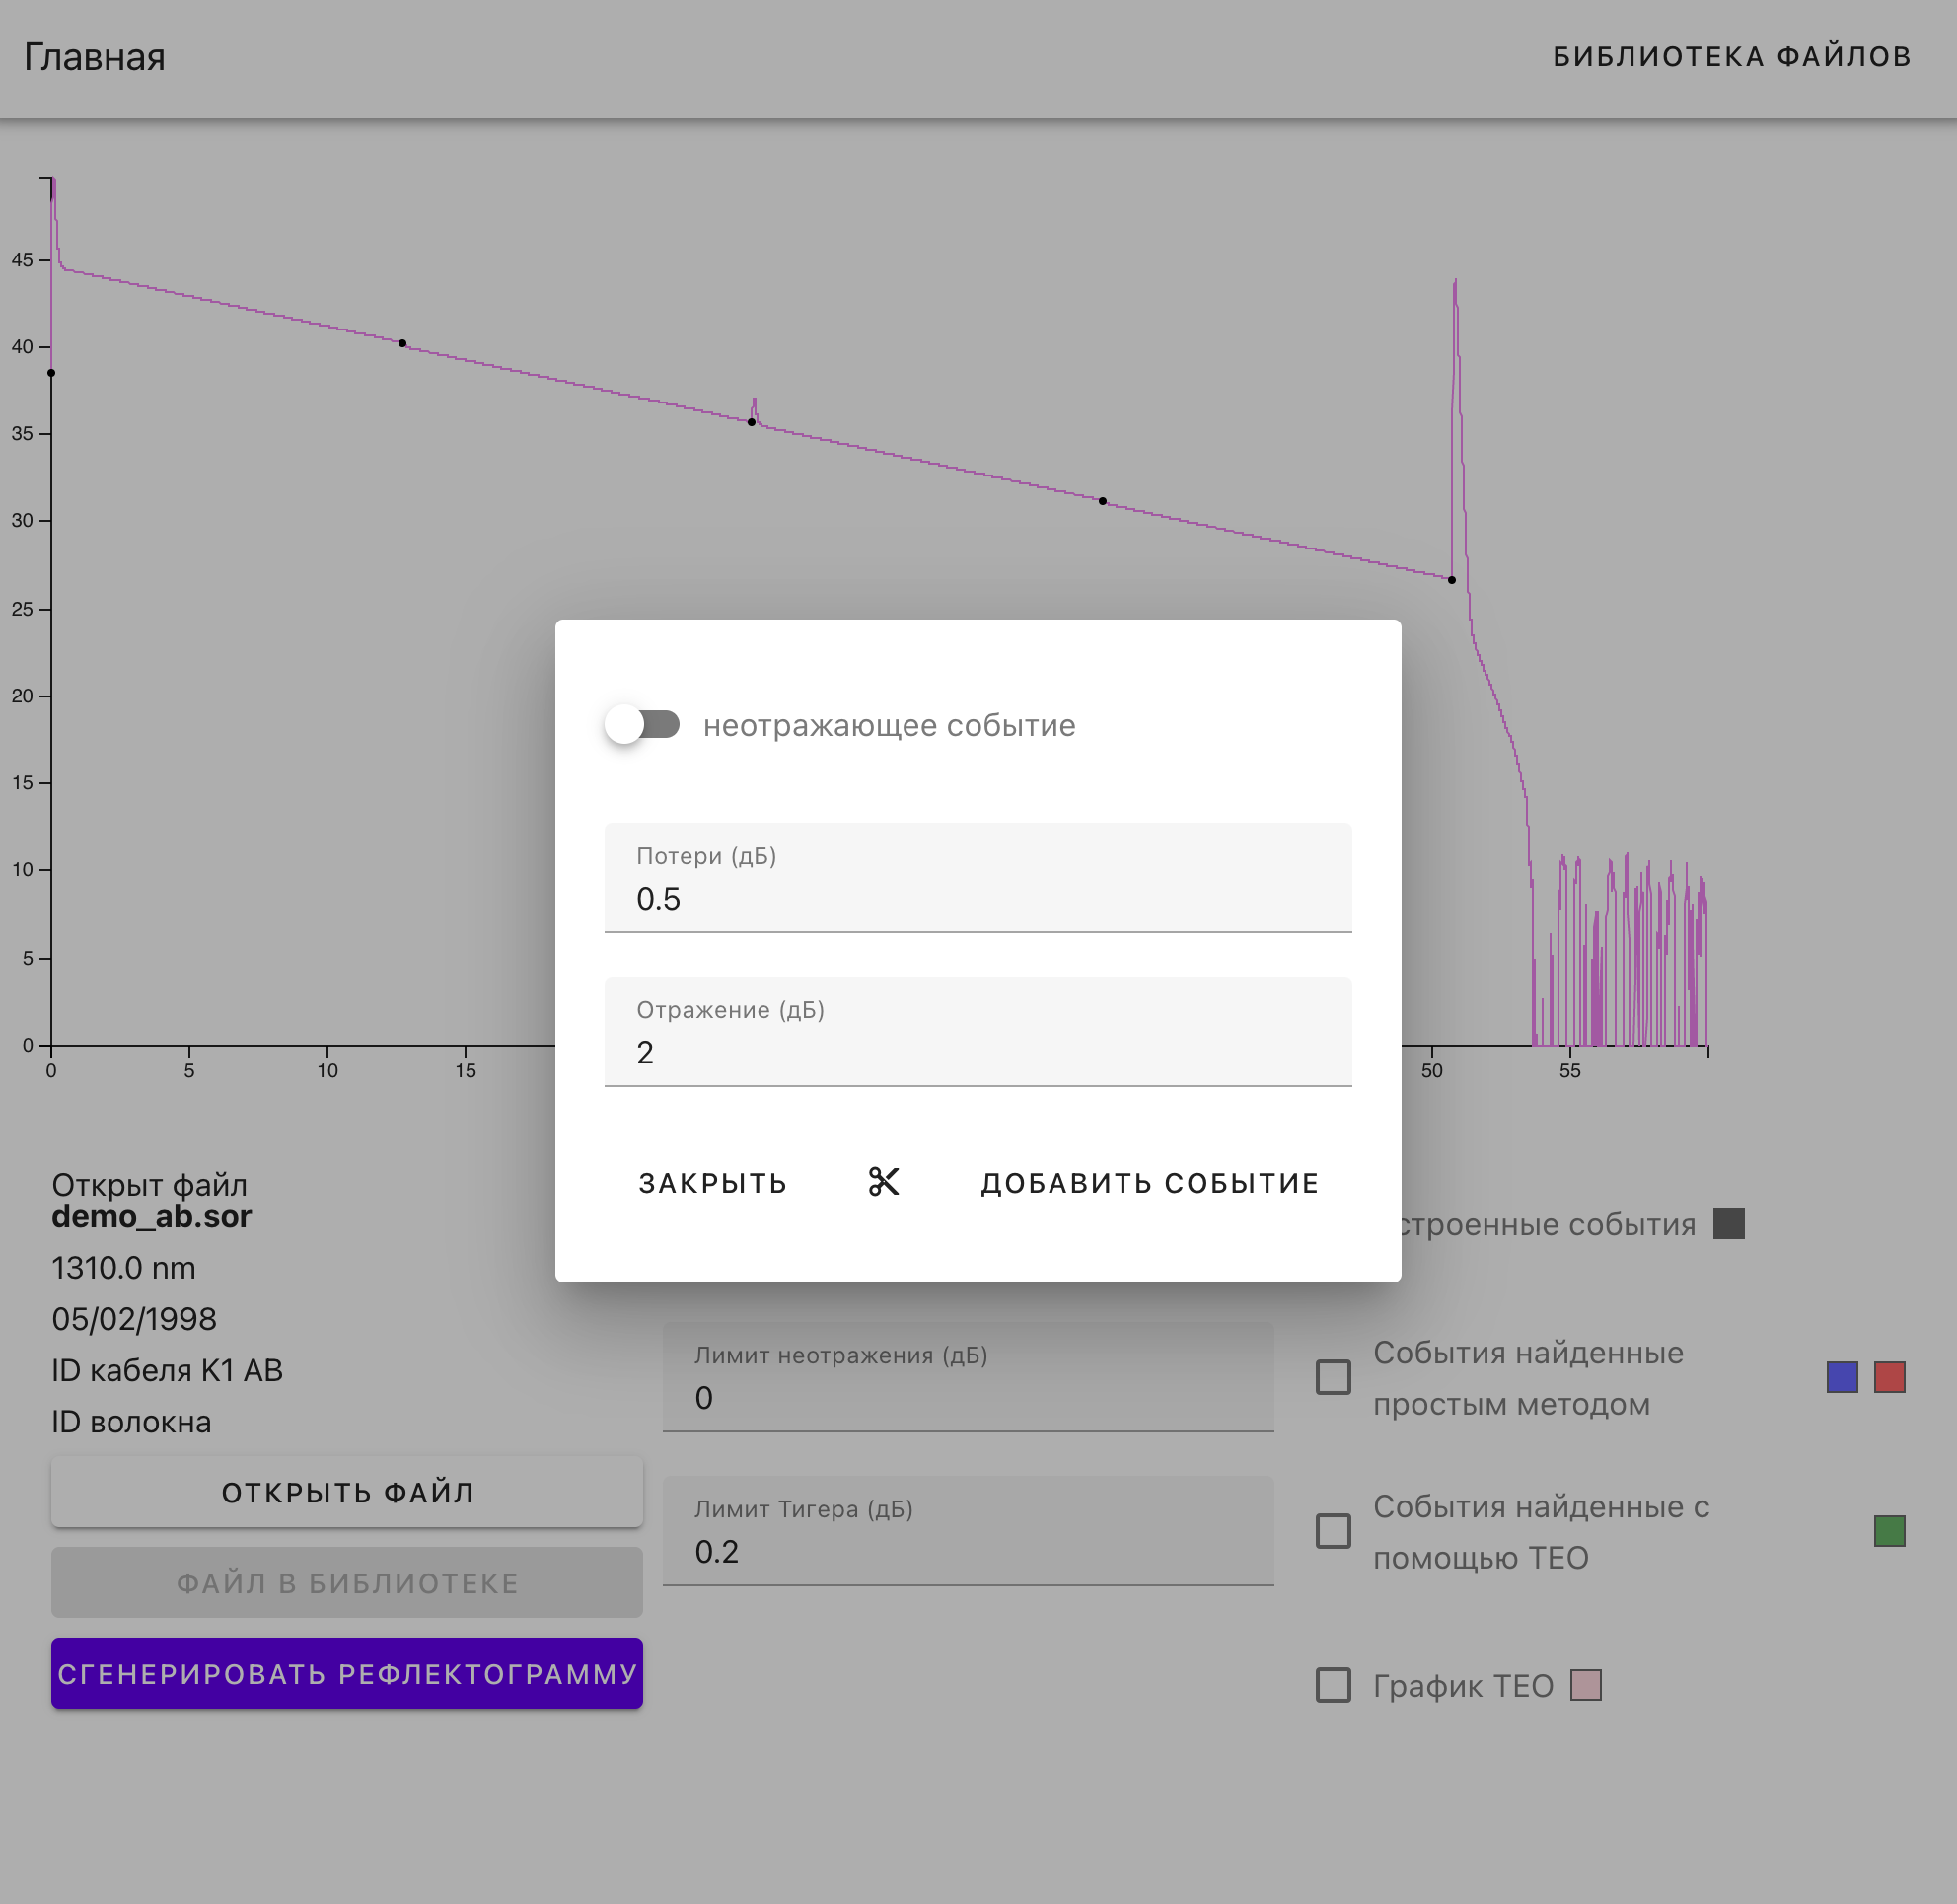
\includegraphics[width=0.65\textwidth]{edit_modal}}}
  \caption{\Gls{модальное окно} редактирования}
  \label{ris:edit_modal}
\end{figure}

\begin{figure}[H]
  \center{\frame{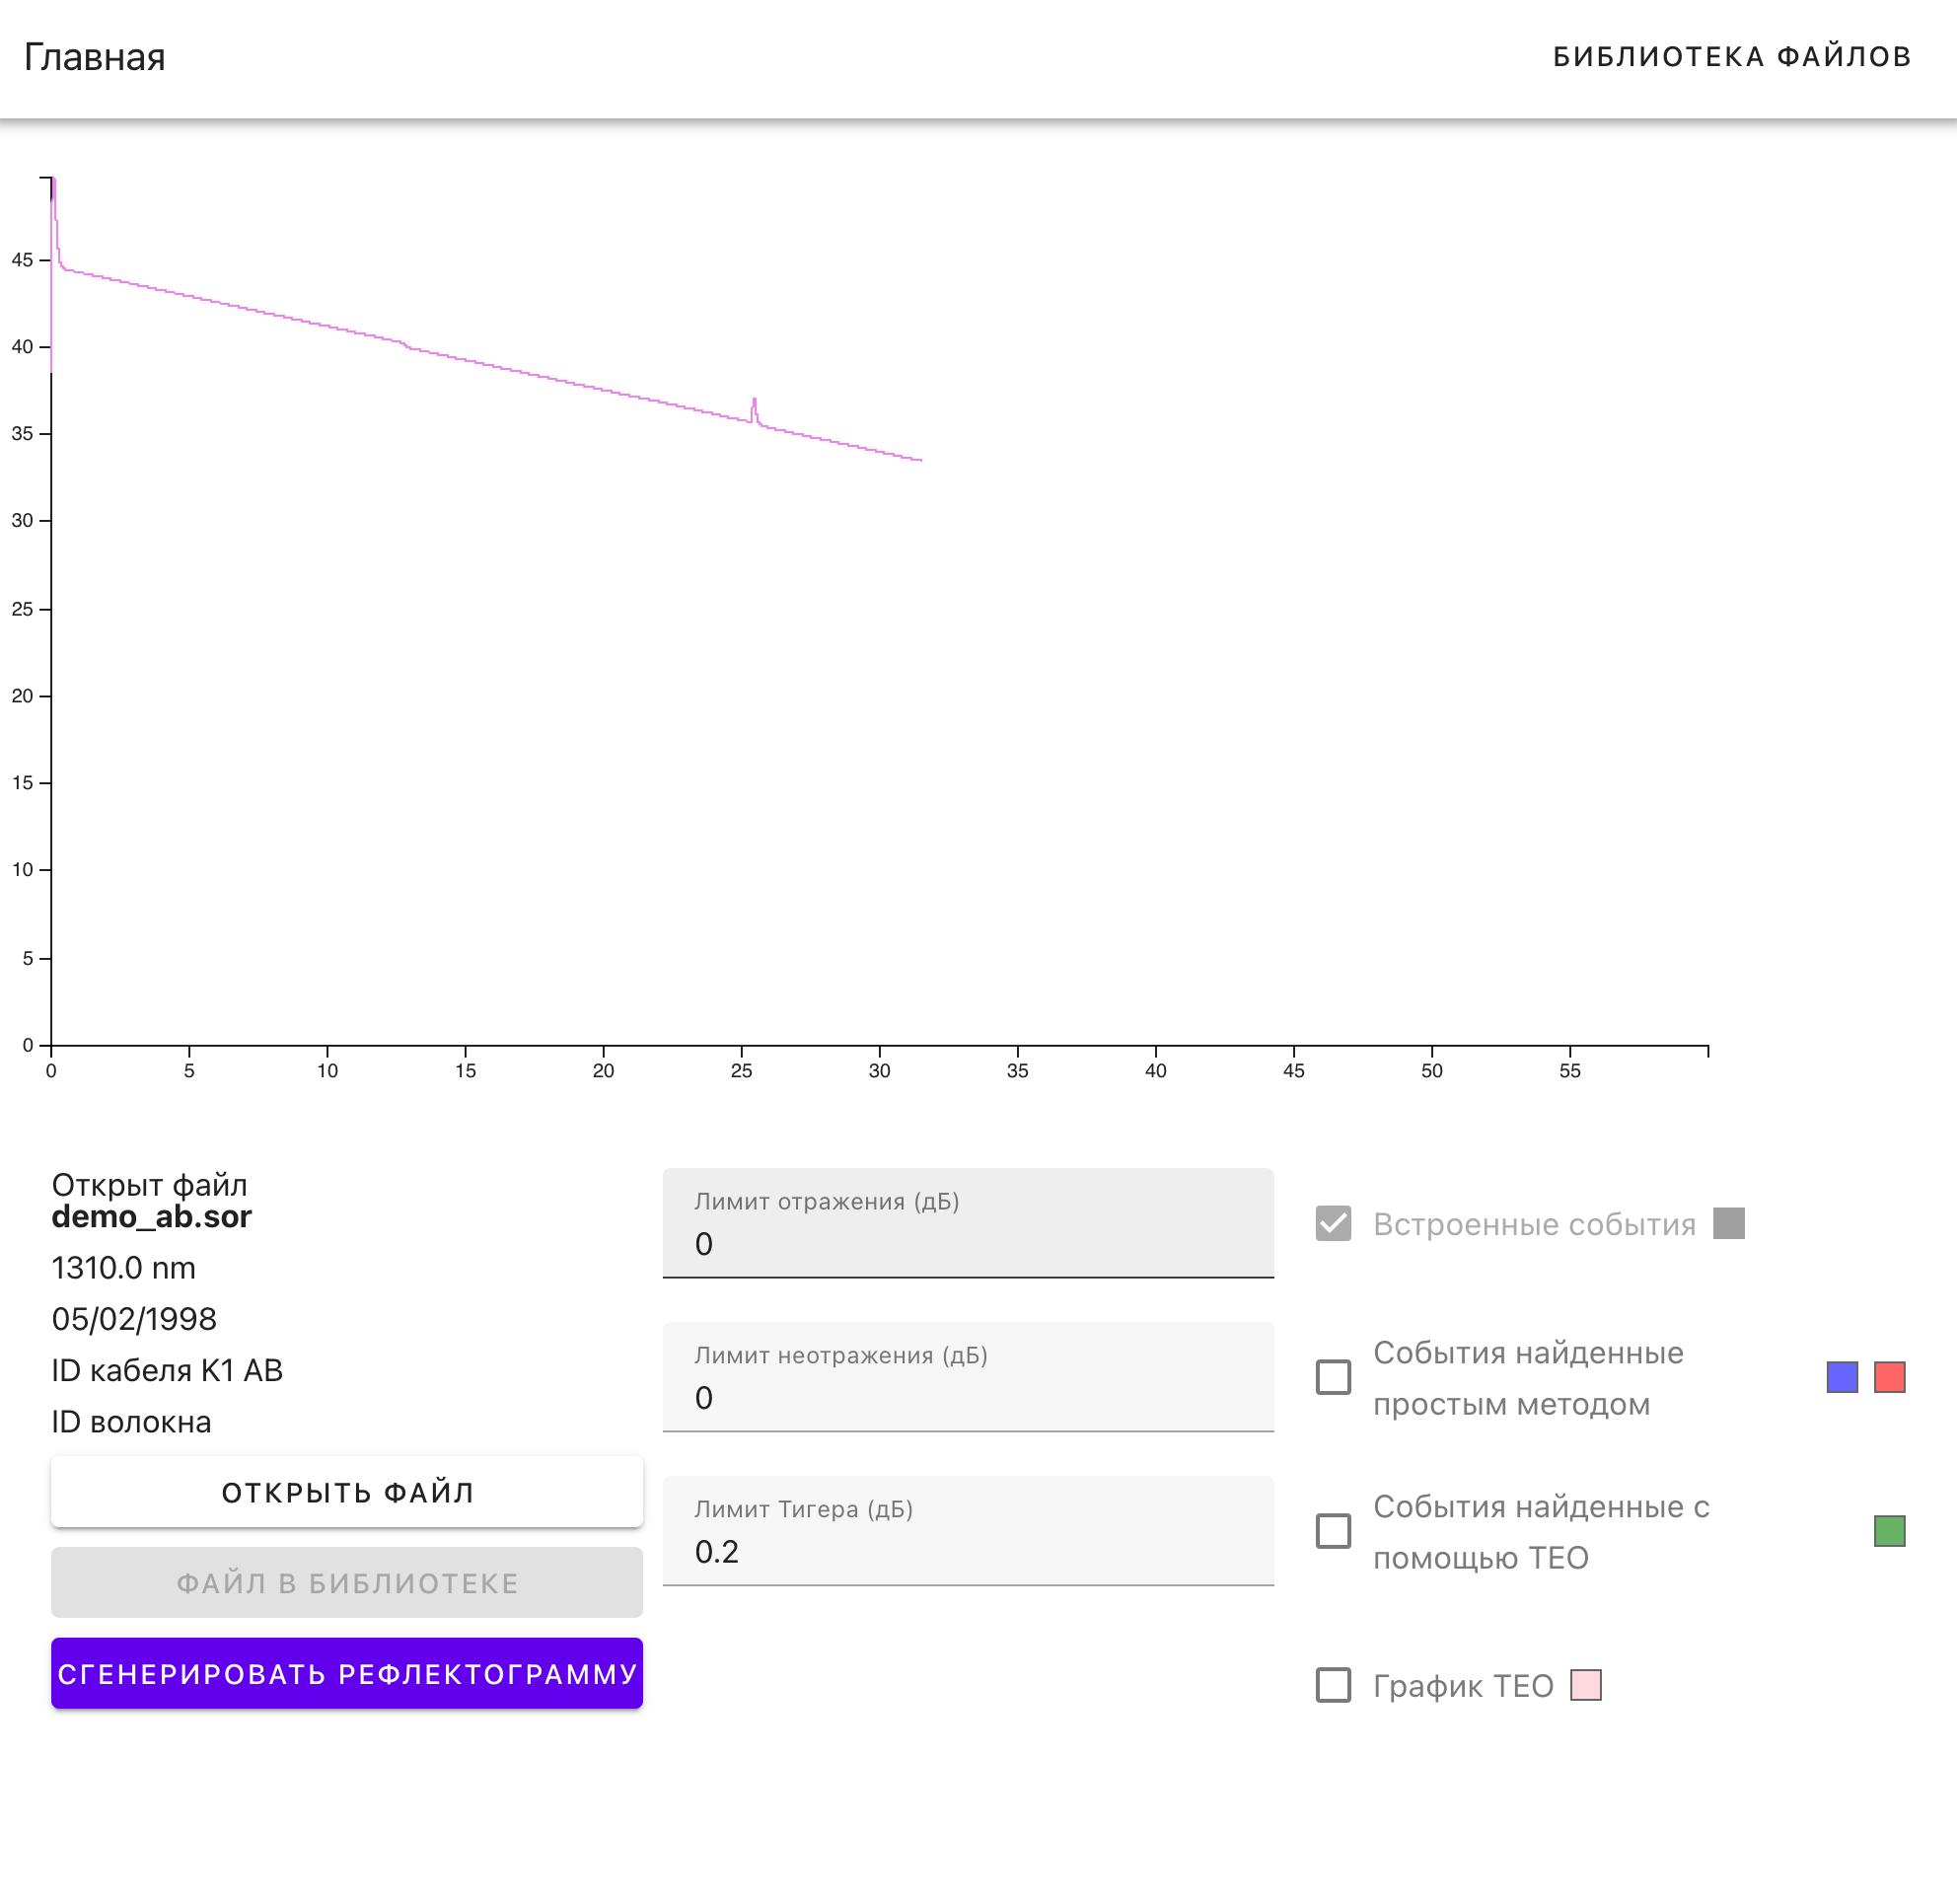
\includegraphics[width=0.65\textwidth]{cut_result}}}
  \caption{Результат выполнения действия <<Обрезка рефлектограммы>>}
  \label{ris:cut_result}
\end{figure}

\begin{figure}[H]
  \center{\frame{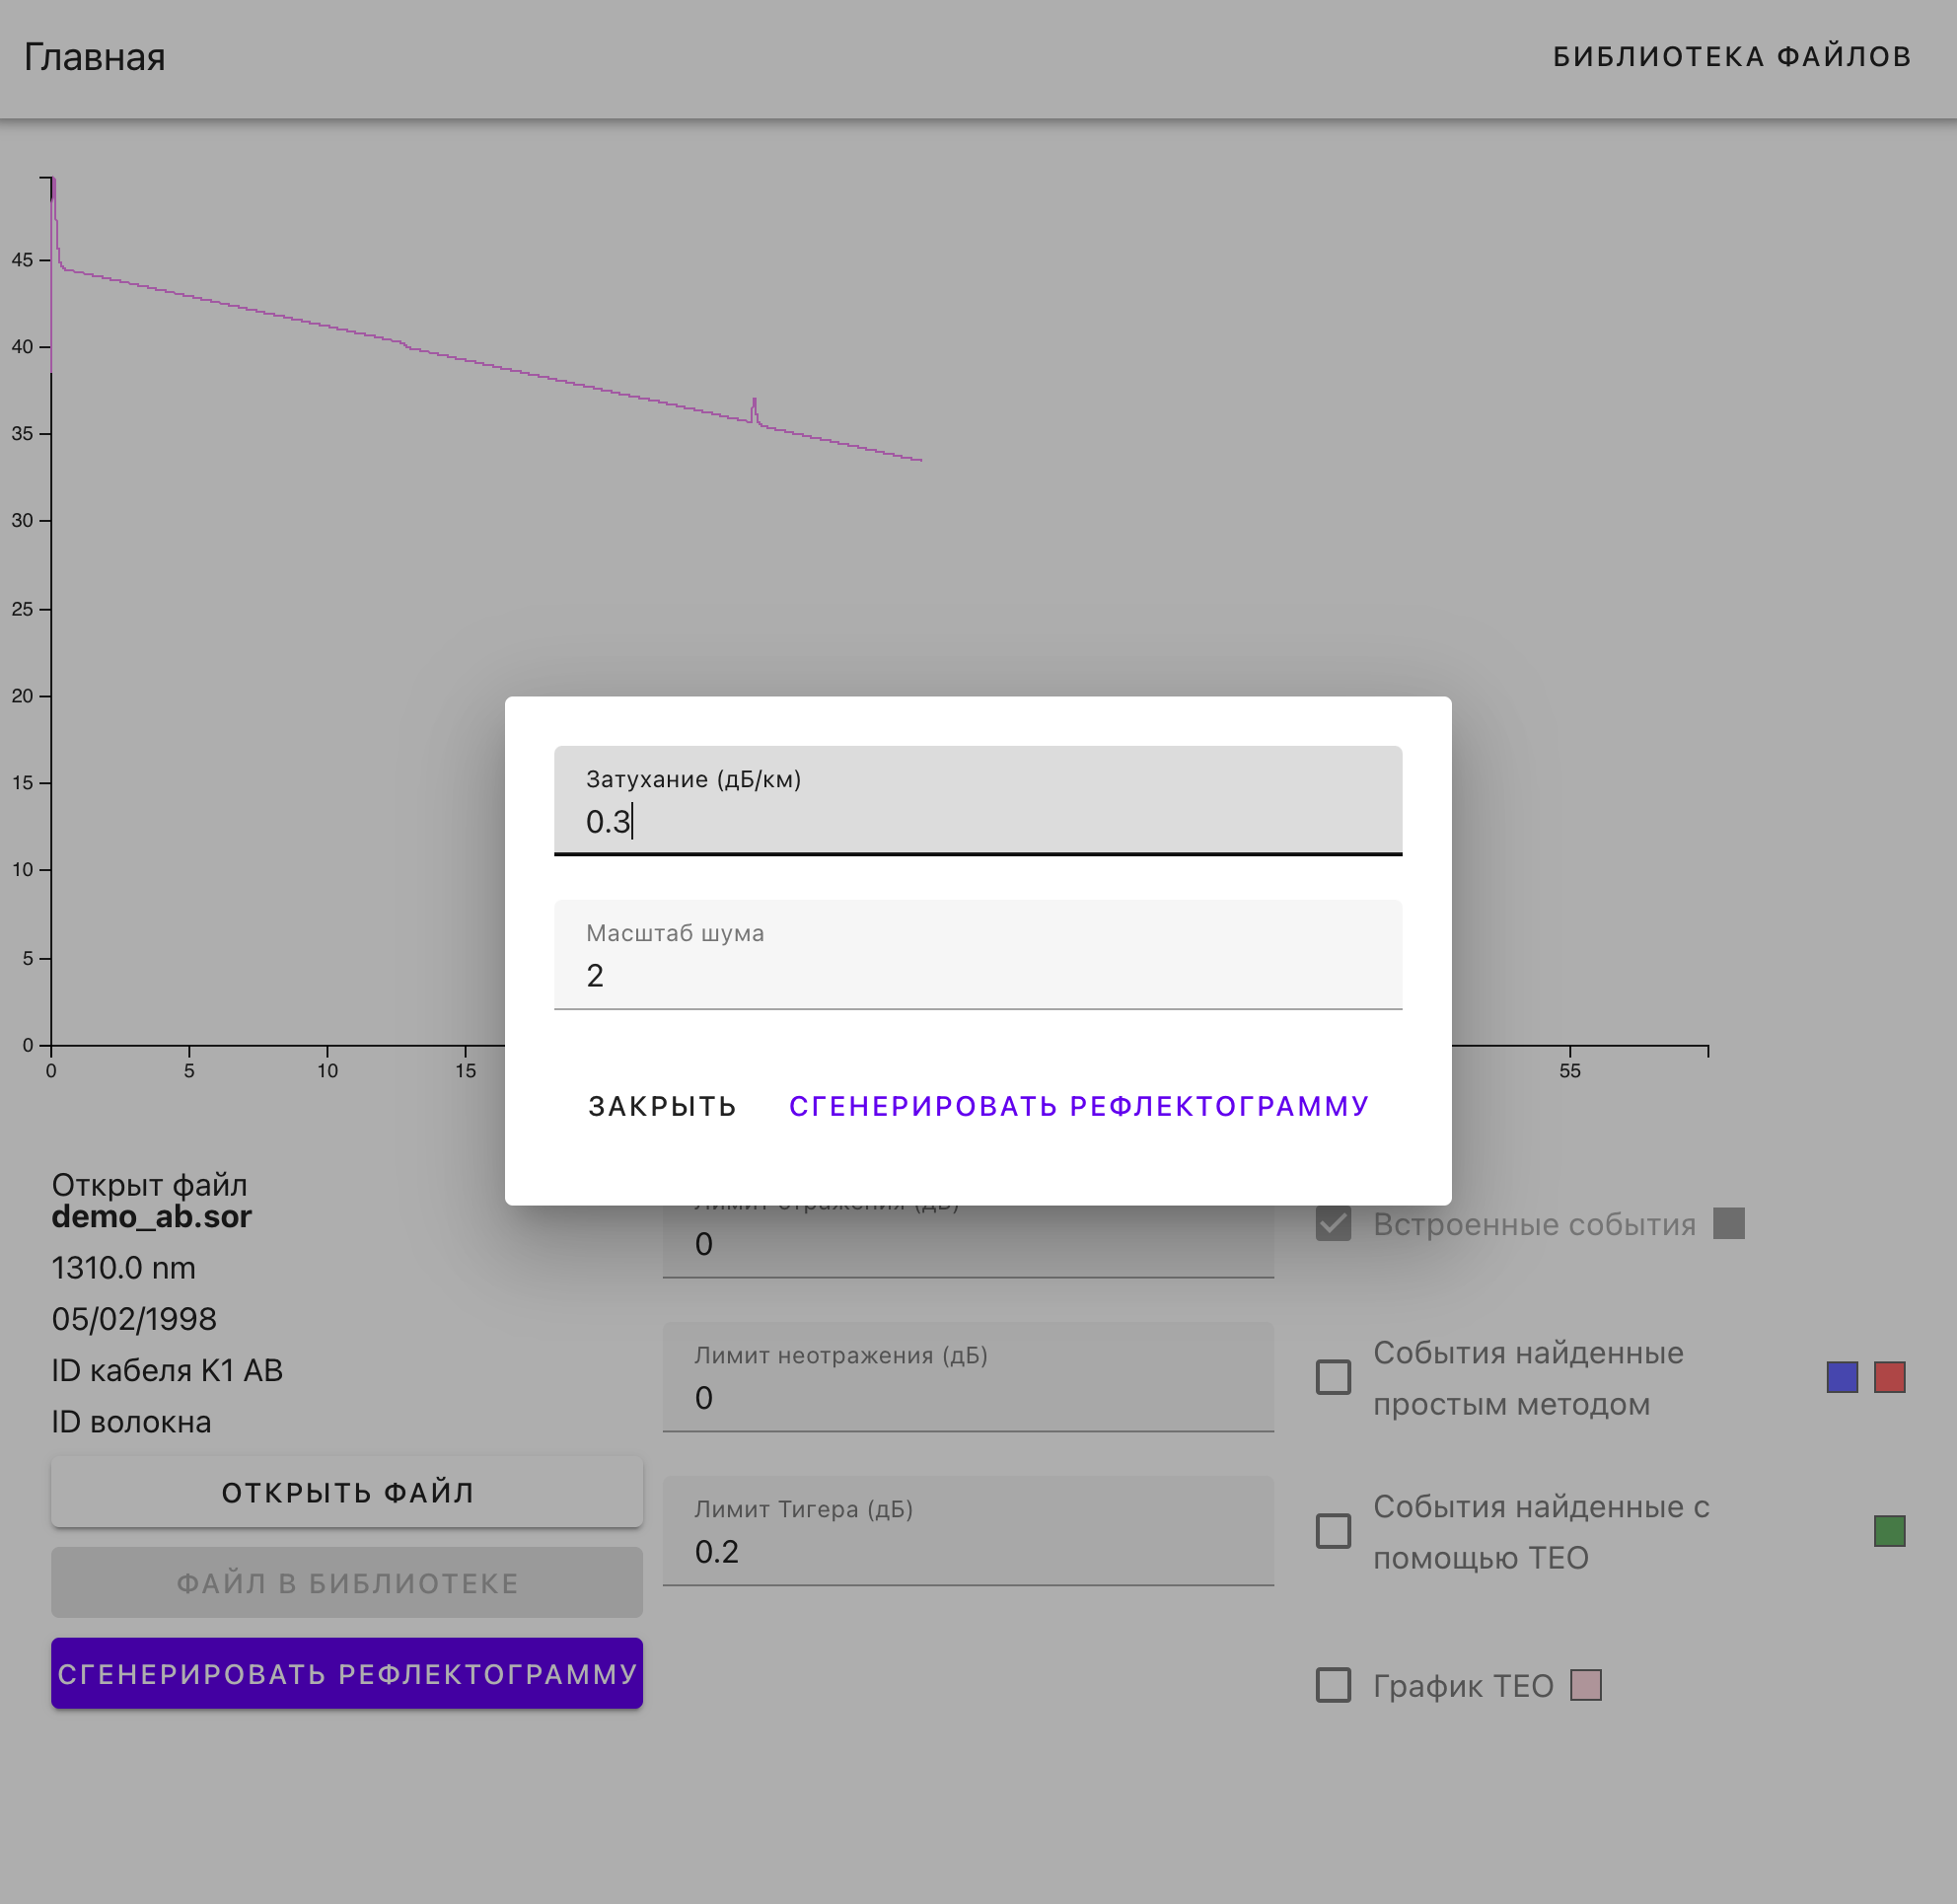
\includegraphics[width=0.65\textwidth]{generate}}}
  \caption{\Gls{модальное окно} <<Сгенерировать рефлектограммму>>}
  \label{ris:generate}
\end{figure}

\begin{figure}[H]
  \center{\frame{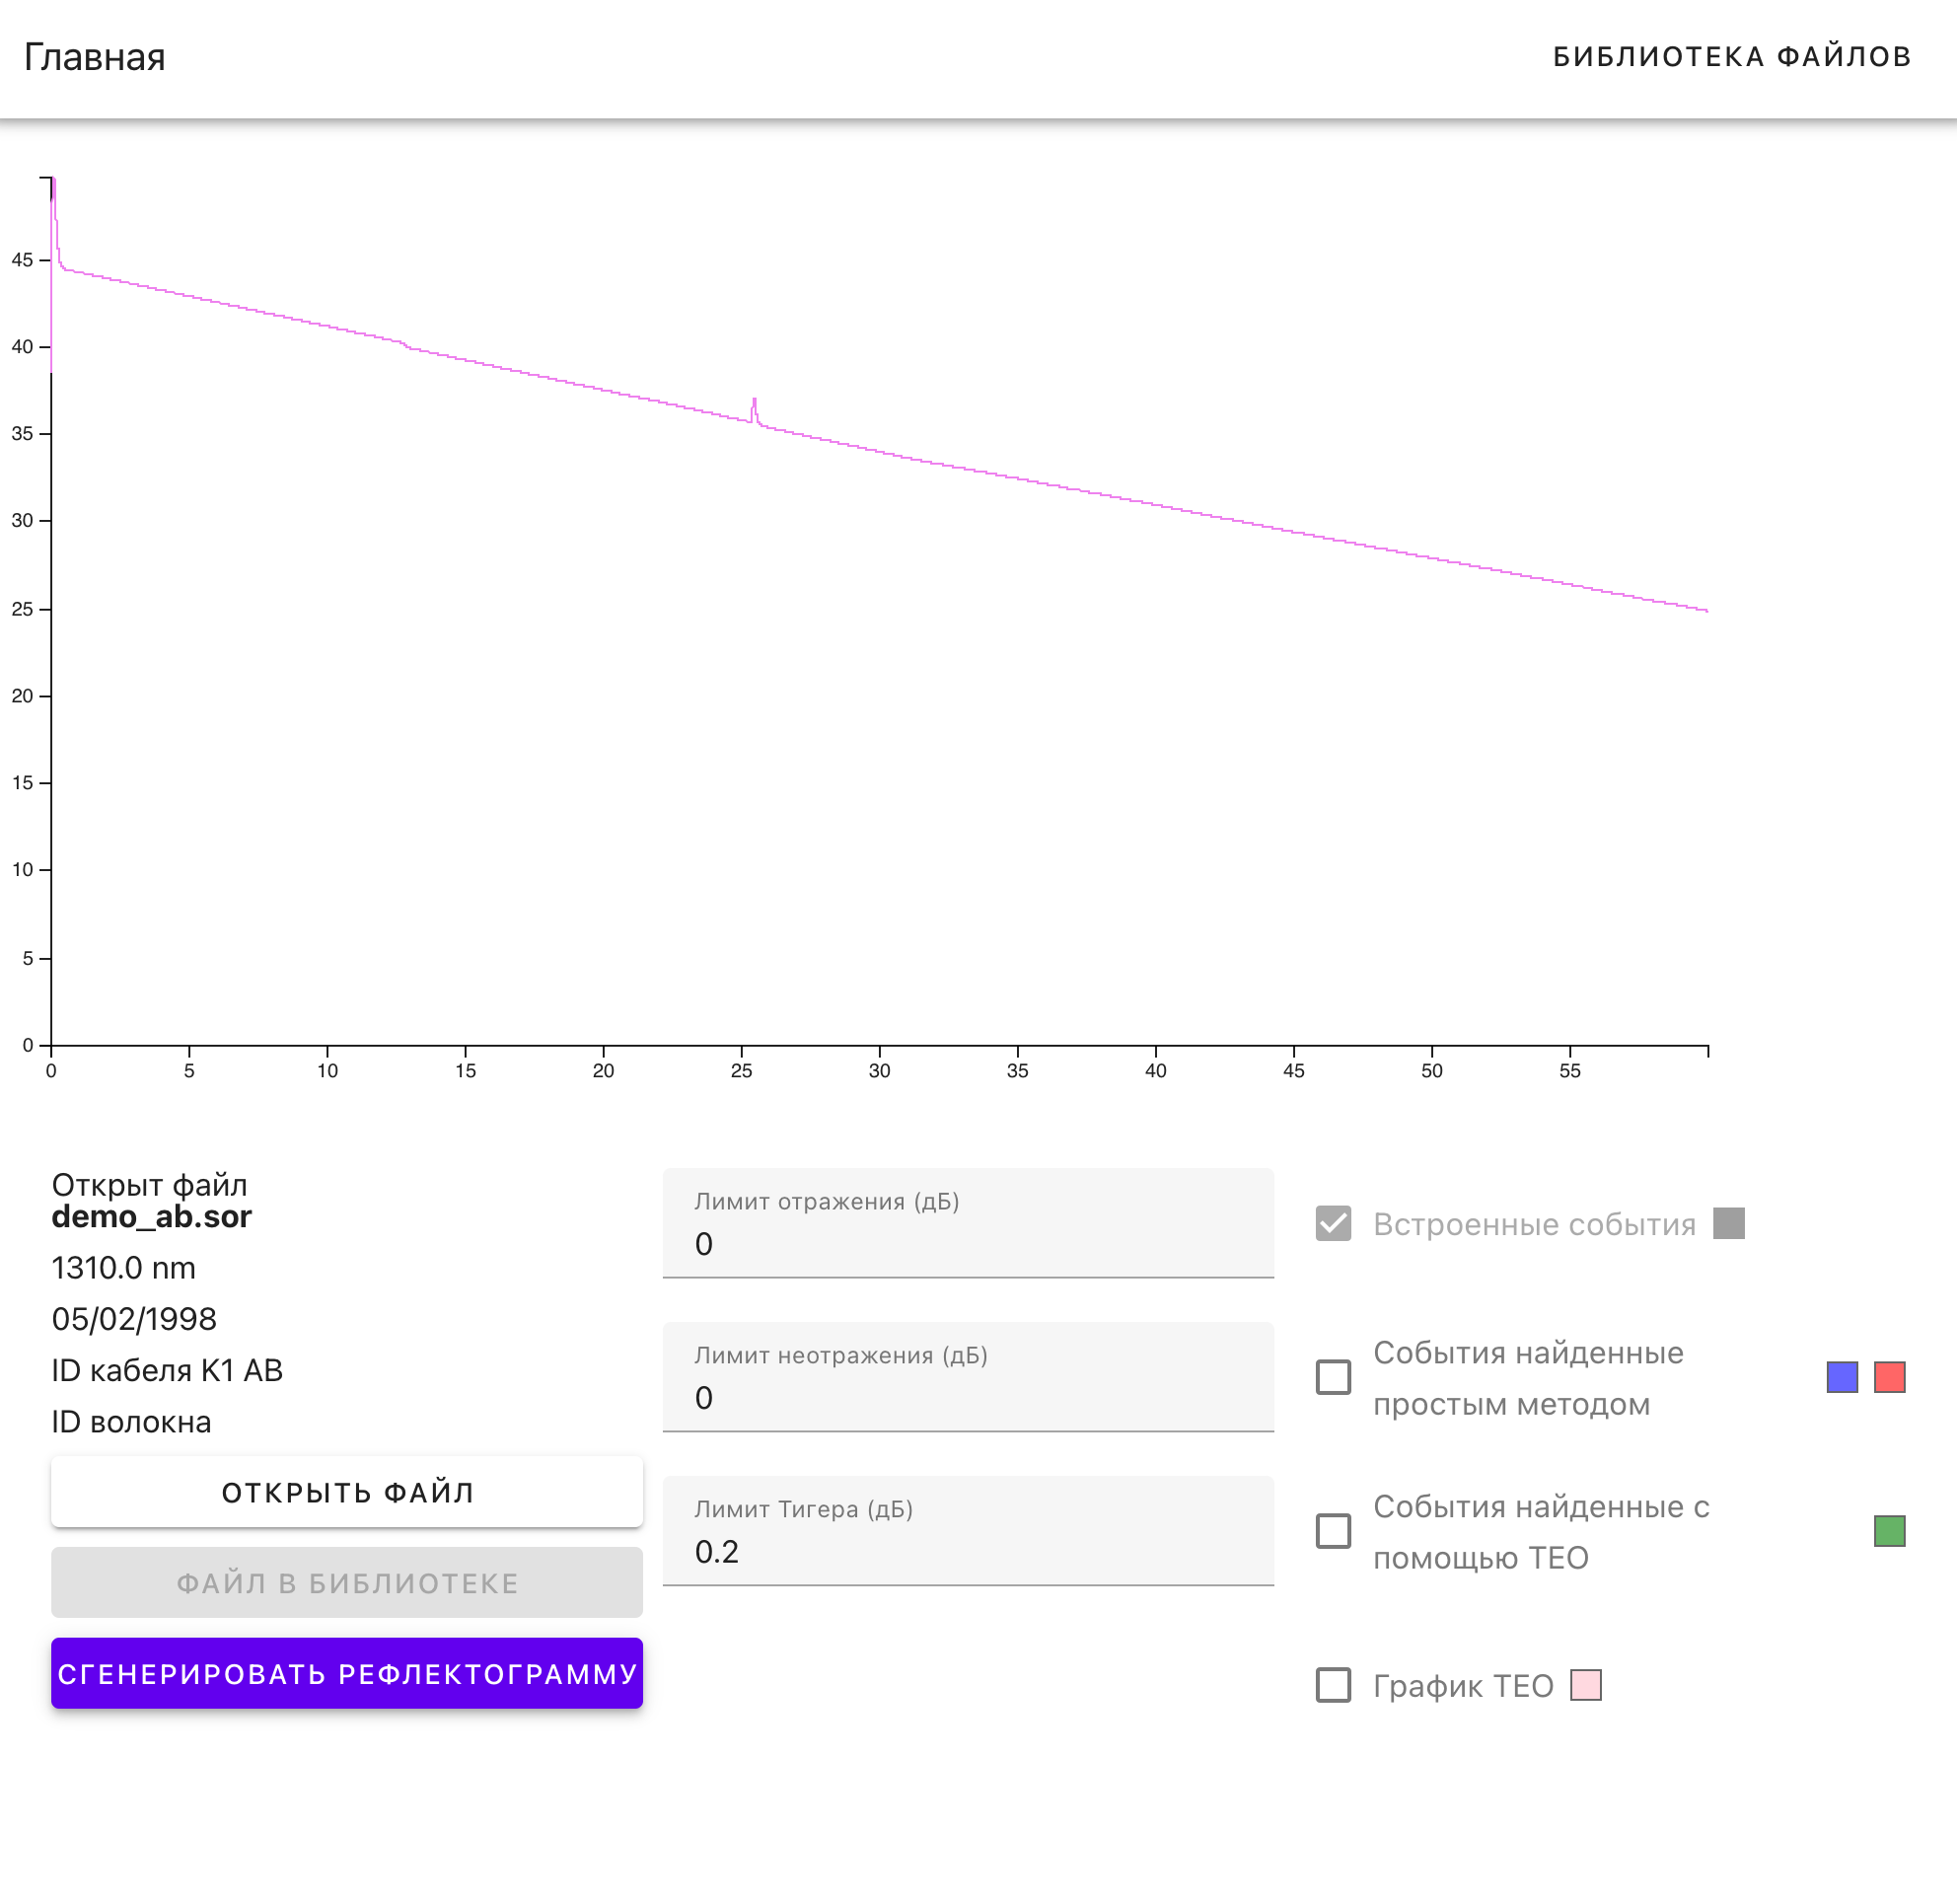
\includegraphics[width=0.65\textwidth]{generate_result}}}
  \caption{Результат выполнения действия <<Сгенерировать рефлектограммму>>}
  \label{ris:generate_result}
\end{figure}

\begin{figure}[H]
  \center{\frame{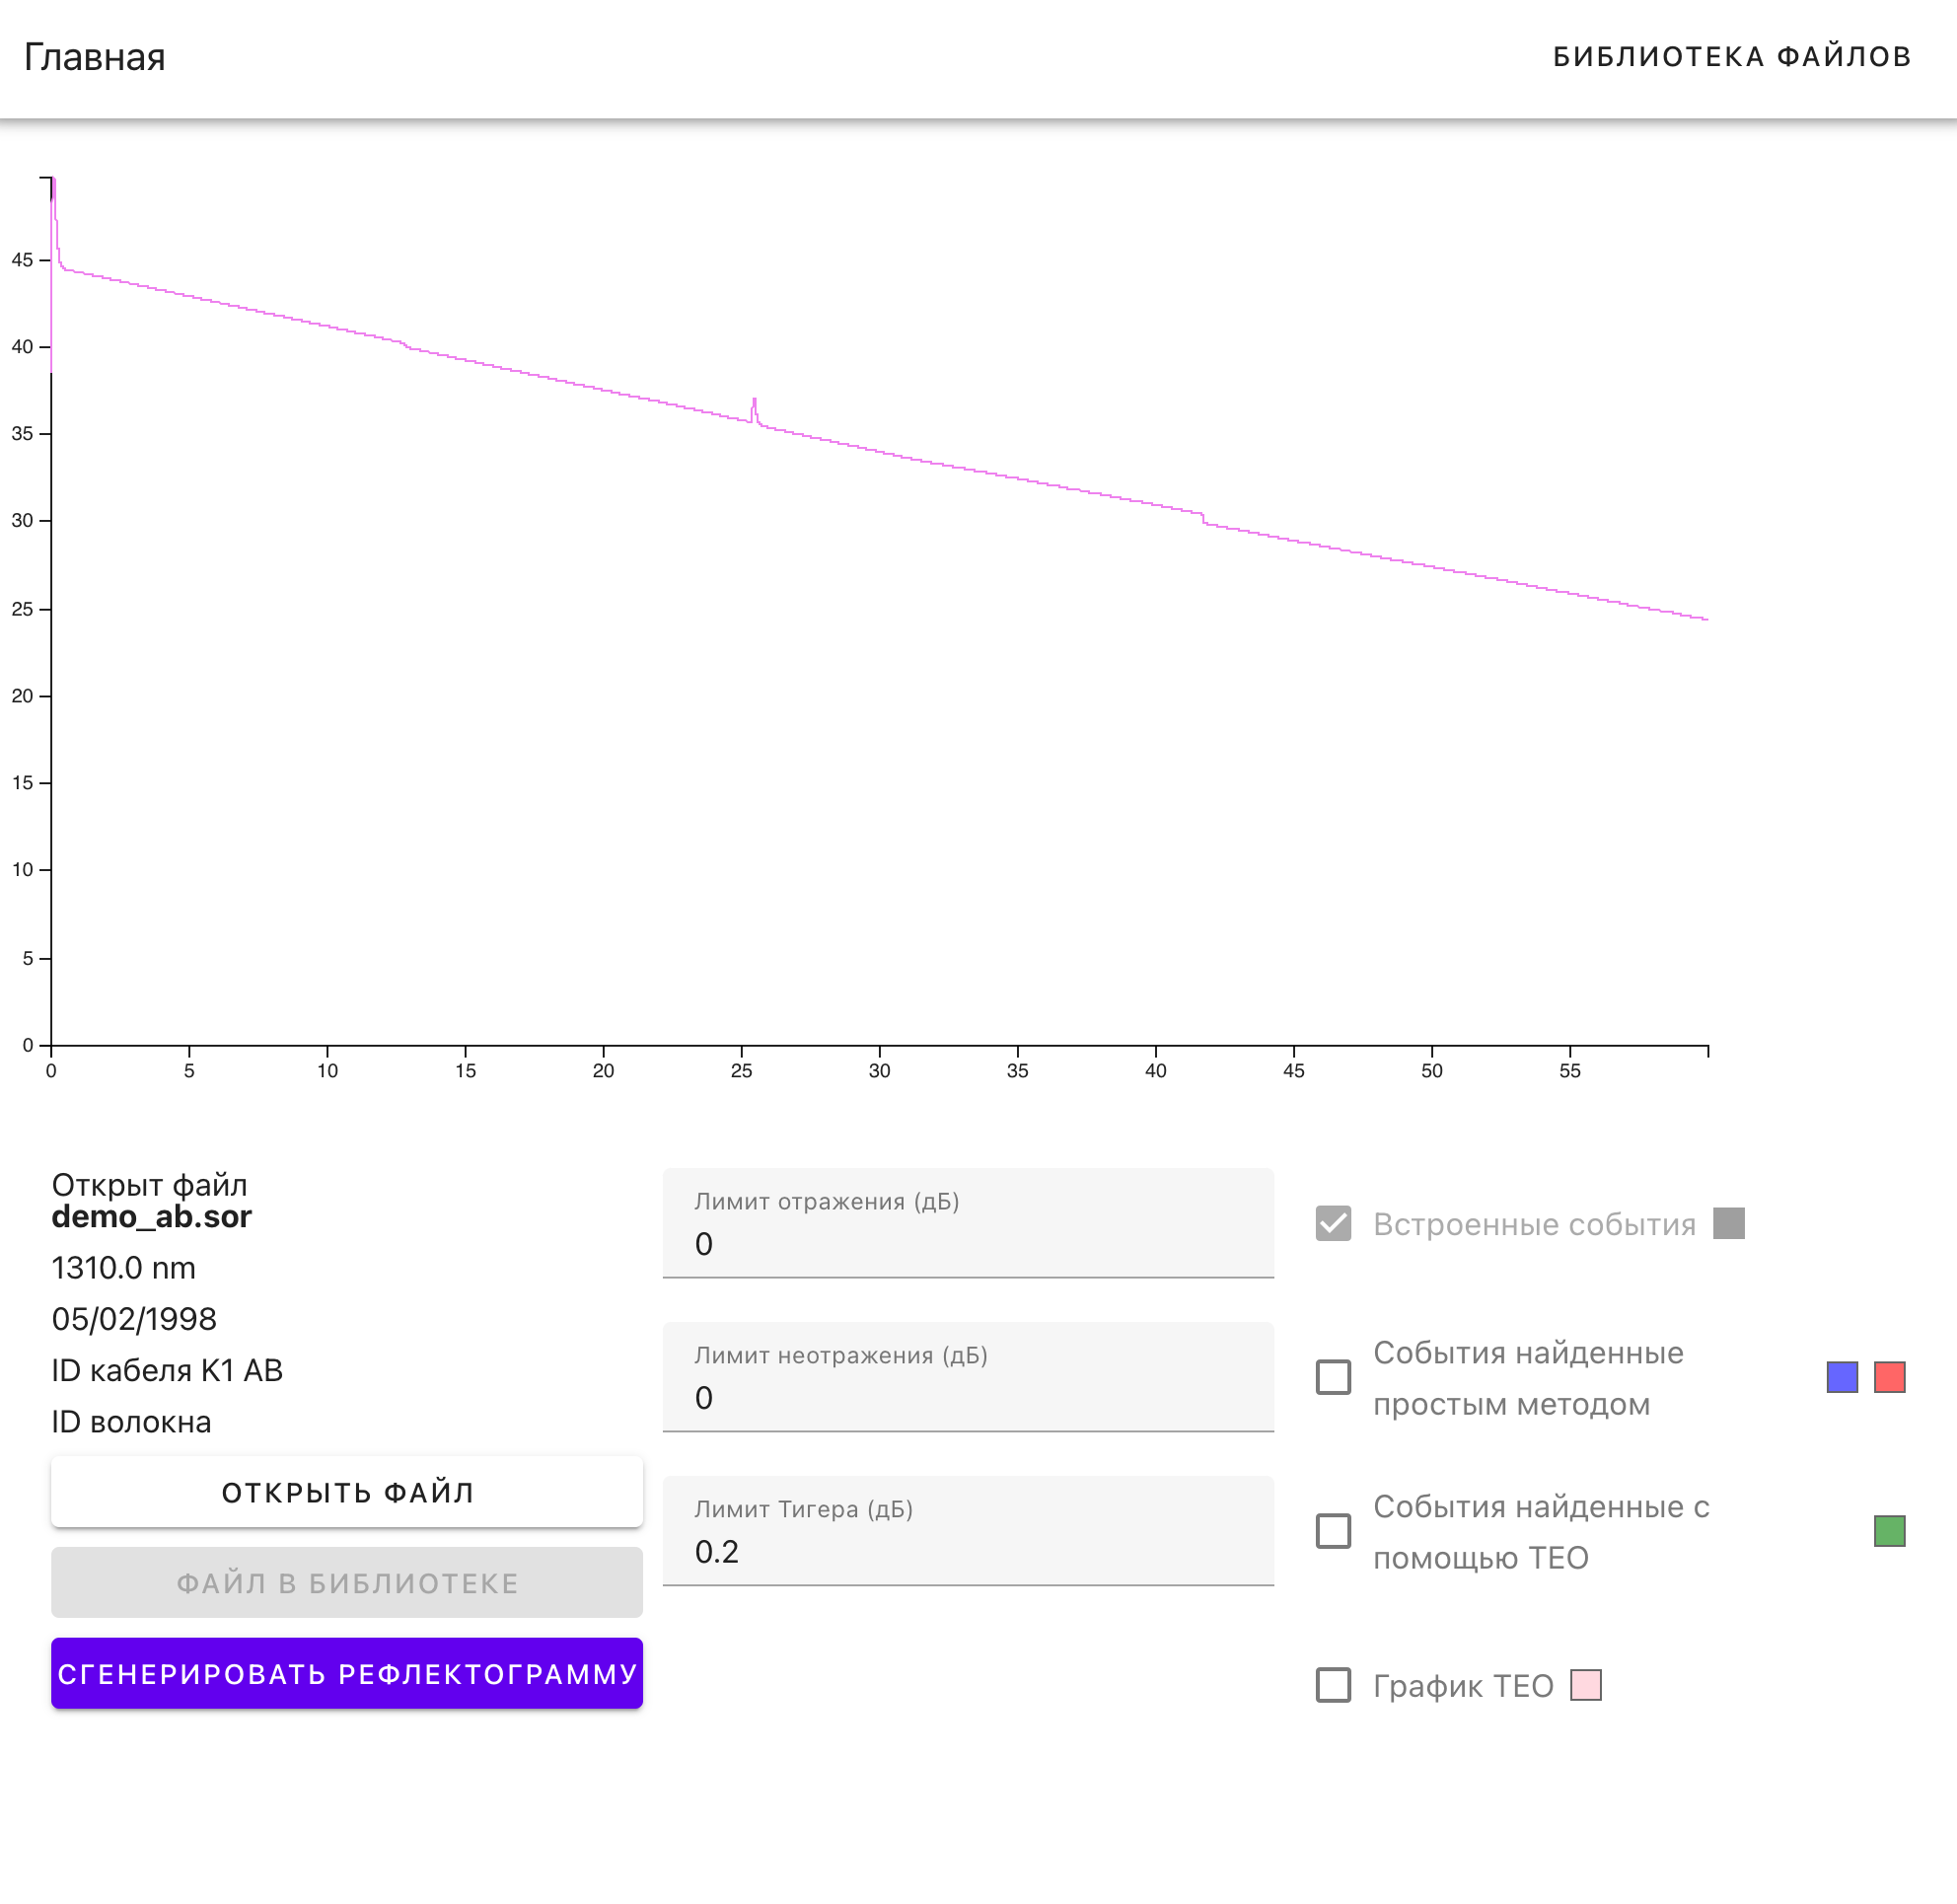
\includegraphics[width=0.65\textwidth]{loss_event_added}}}
  \caption{Результат выполнения действия <<Добавить событие>> с параметром <<Неотражающее событие>>}
  \label{ris:loss_event_added}
\end{figure}

\begin{figure}[H]
  \center{\frame{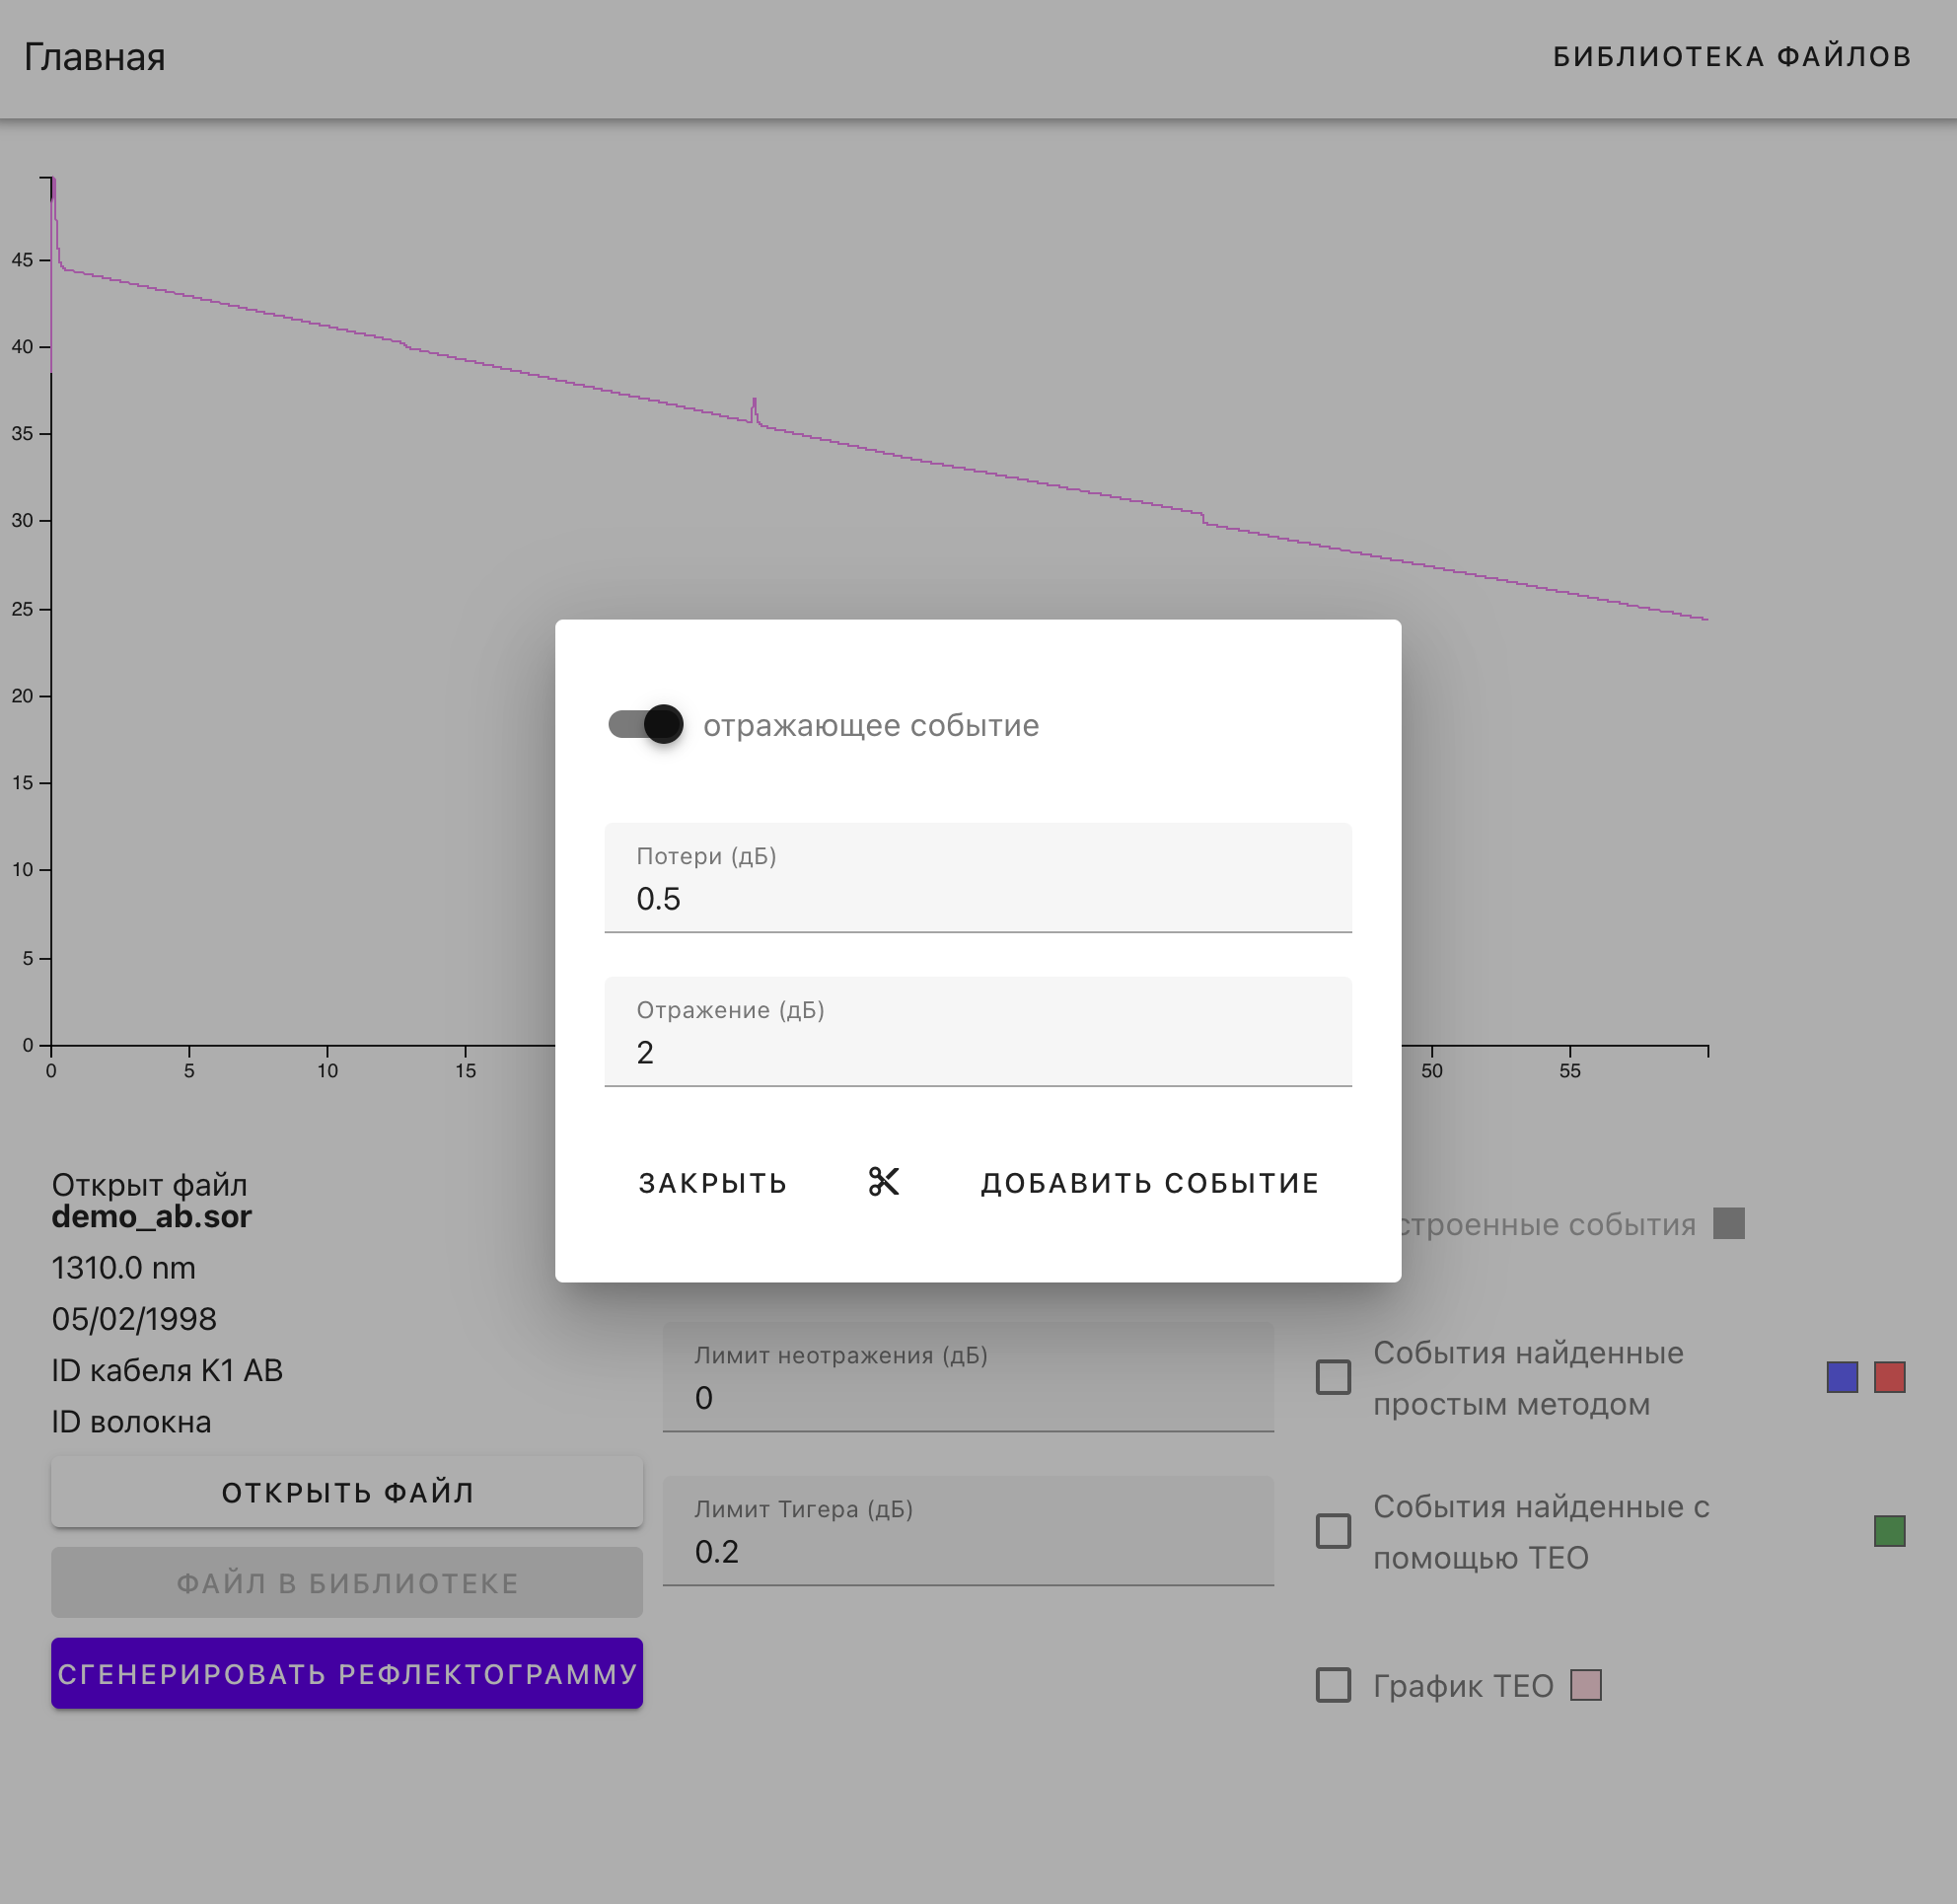
\includegraphics[width=0.65\textwidth]{edit_modal_reflection}}}
  \caption{\Gls{модальное окно} редактирования с селектором в положении <<Отражающее событие>>}
  \label{ris:edit_modal_reflection}
\end{figure}

\begin{figure}[H]
  \center{\frame{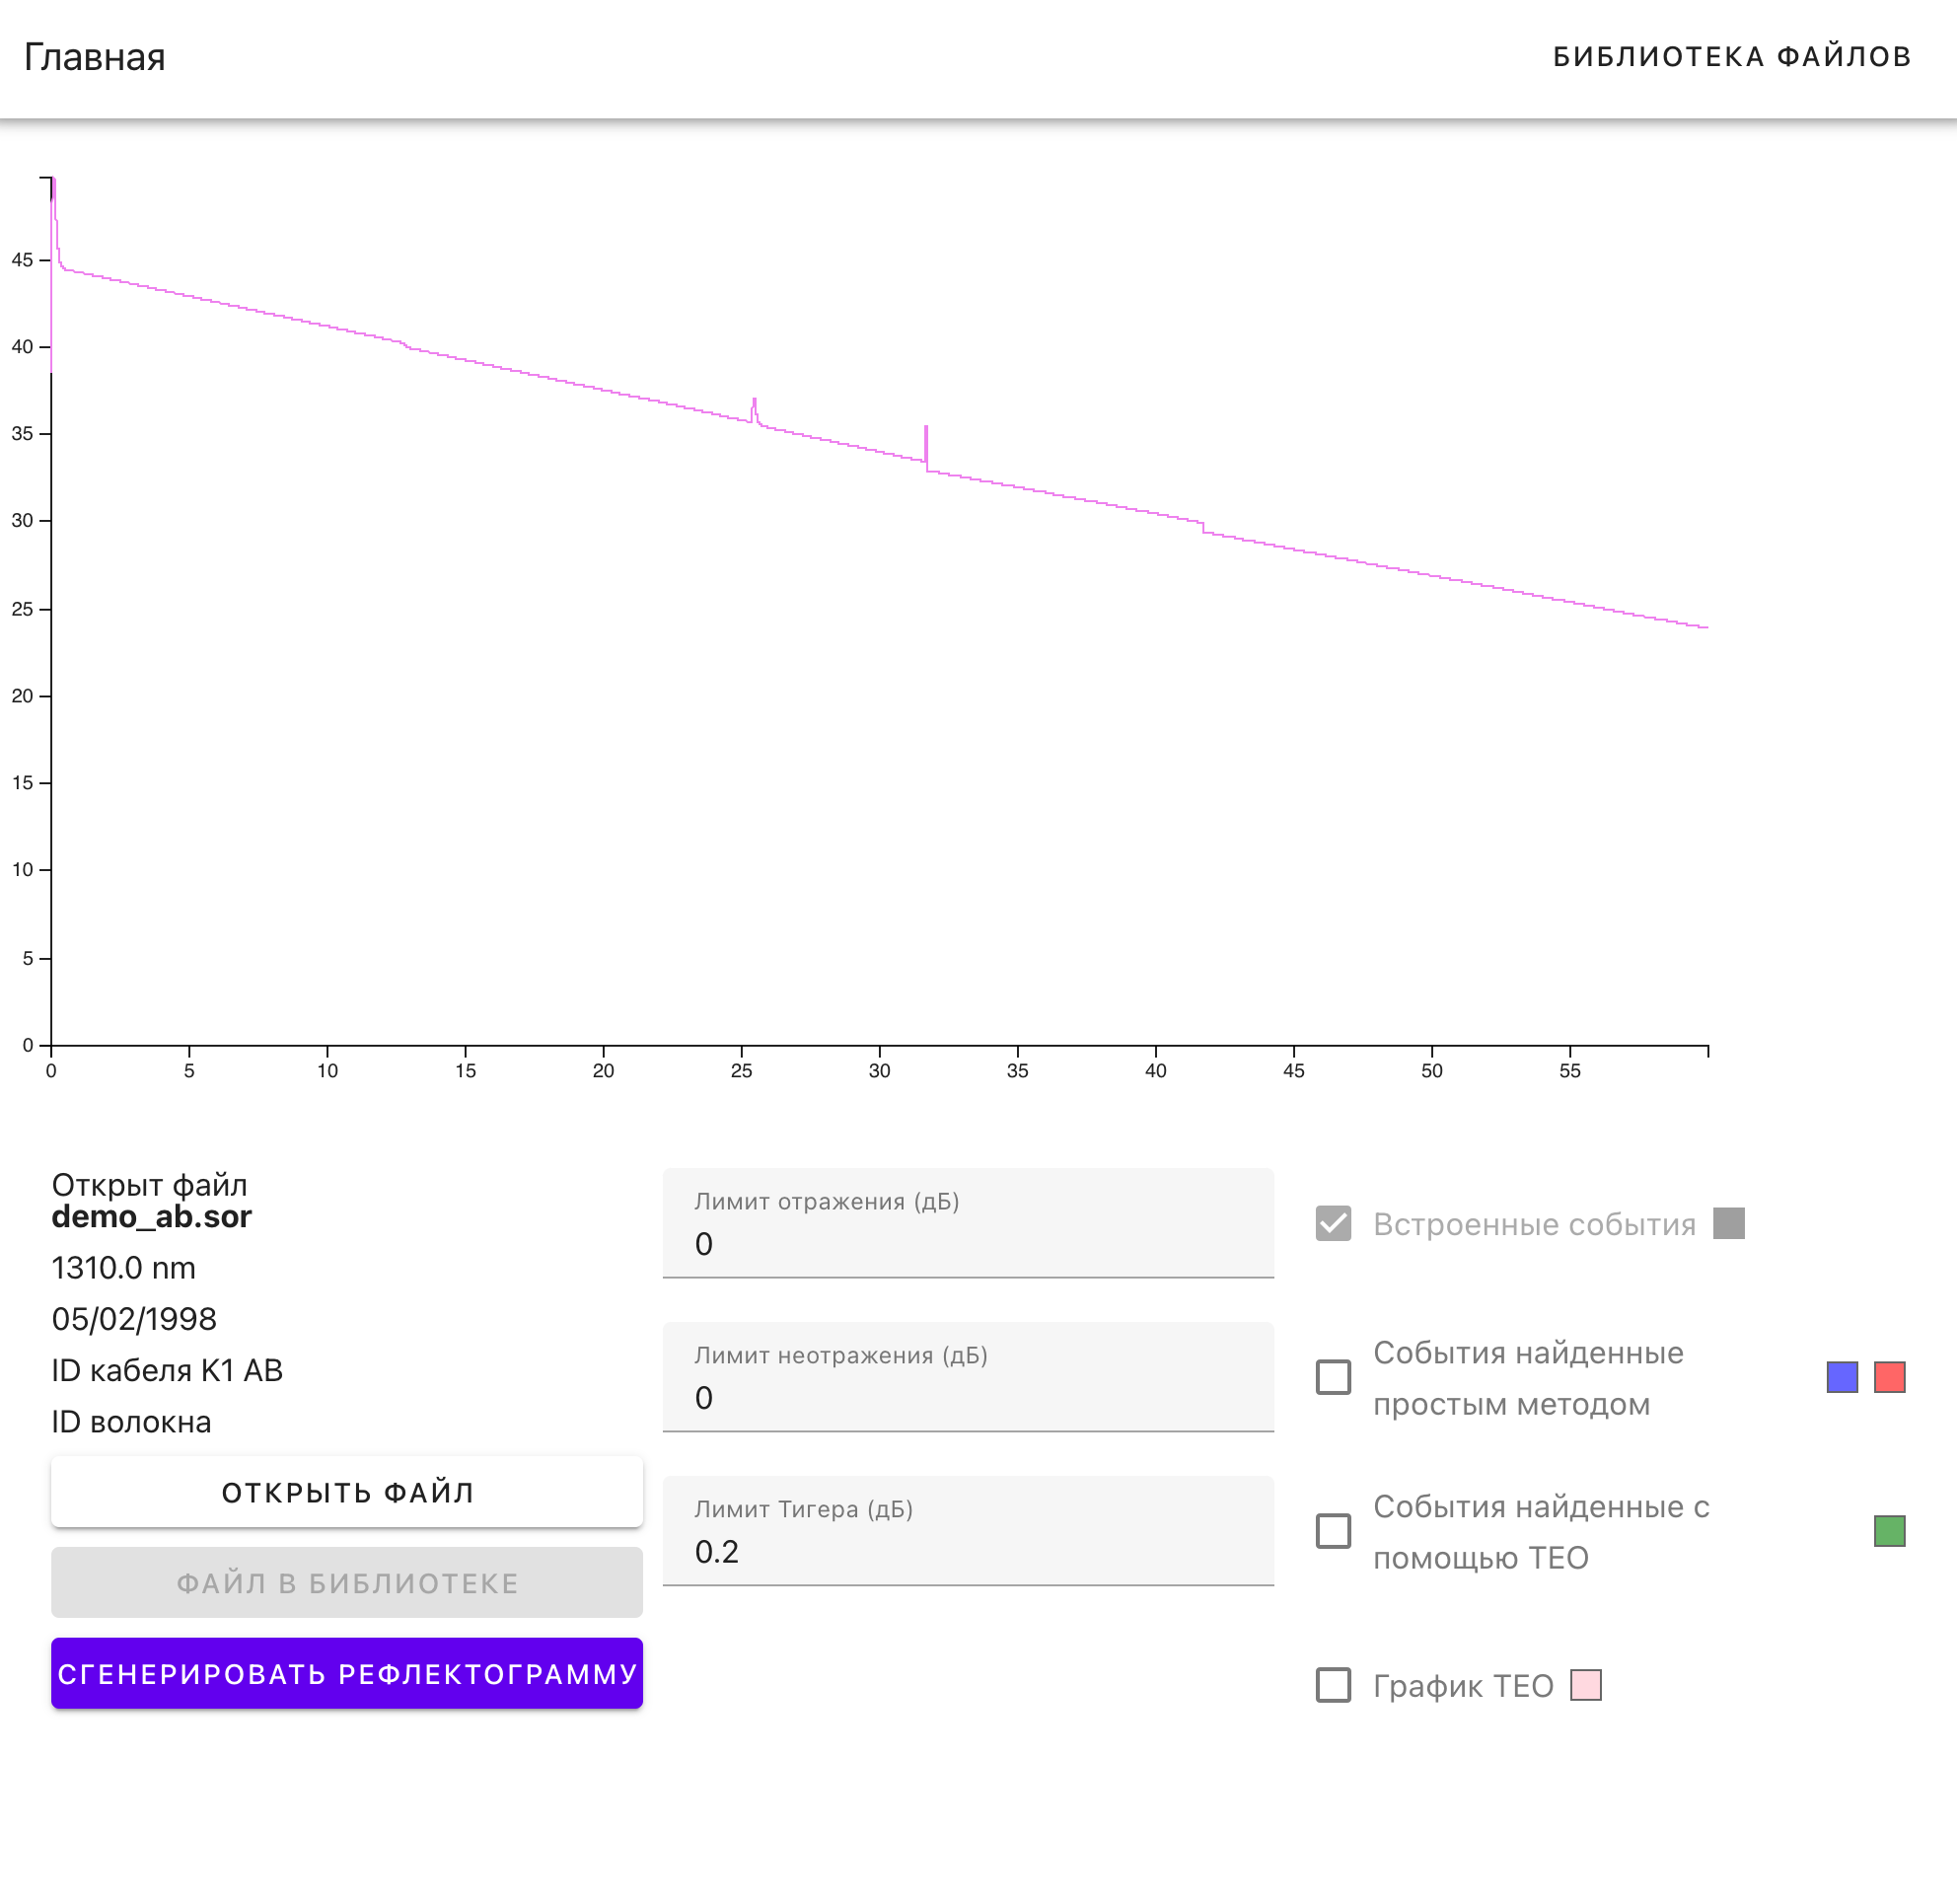
\includegraphics[width=0.65\textwidth]{reflection_event_added}}}
  \caption{Результат выполнения действия <<Добавить событие>> с параметром <<Отражающее событие>>}
  \label{ris:reflection_event_added}
\end{figure}

\begin{figure}[H]
  \center{\frame{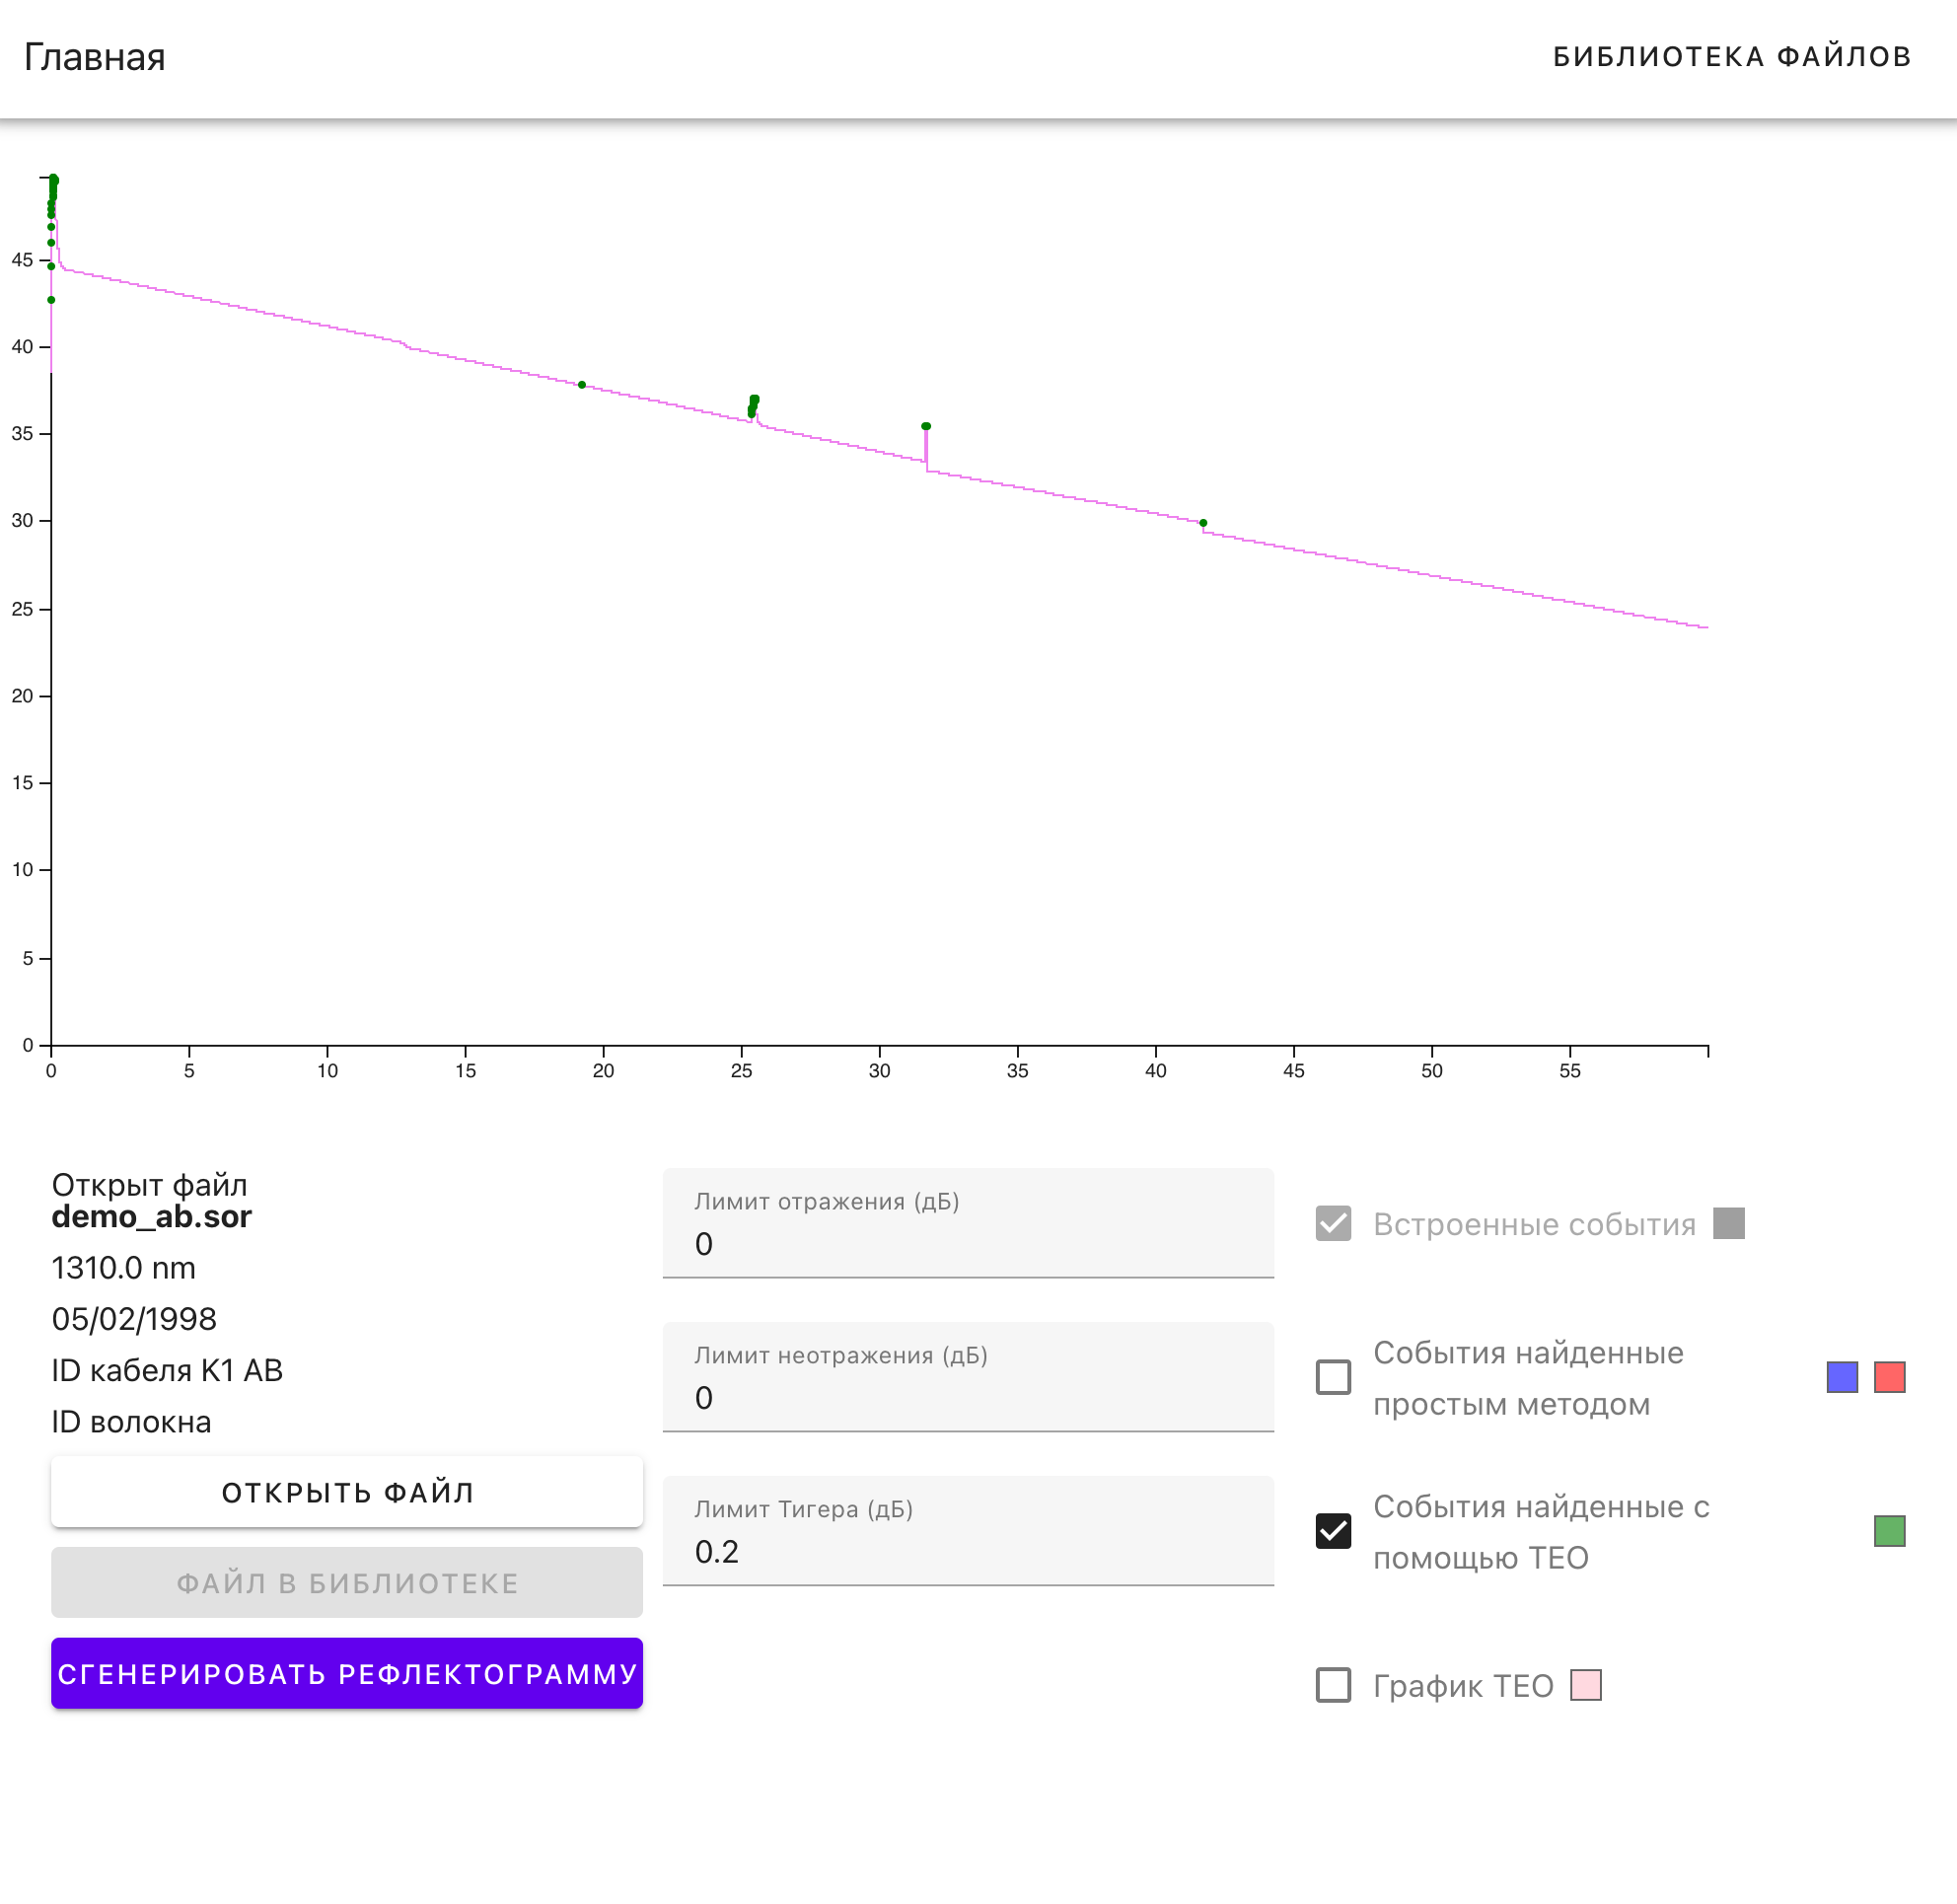
\includegraphics[width=0.65\textwidth]{events_after_editing}}}
  \caption{Поиск событий на отредактированной рефлектограмме}
  \label{ris:events_after_editing}
\end{figure}

\subsection{Выводы по разделу}

В разделе проведен подробный обзор приложения, продемонстрирована работа всех функций приложения.
